	

\documentclass[10pt,a4paper]{article}
\usepackage[utf8]{inputenc}
\usepackage[english]{babel}
\usepackage{amsmath}
\usepackage{amsfonts}
\usepackage{amssymb}
\usepackage{graphicx}
\usepackage{caption}
\usepackage{float}
\usepackage{array}
\usepackage{booktabs}	% for horizontal lines
\usepackage{varwidth}% http://ctan.org/pkg/varwidth
\usepackage{csvsimple} % automatic table generation from csv files
\usepackage{comment}
\usepackage[style=draft, backend=bibtex]{biblatex}

% Macros zum Setzen von Formeln
%-------------------------------

\newcommand{\gradient}[1]{\left(\nabla #1 \right)}
\newcommand{\hesse}[1]{\left(\nabla^2 #1 \right)}
 
% transponiert
\newcommand{\transpose}[1]{#1^\mathrm{T}}
% Exponentialfunktion
\newcommand{\e}{\mathrm{e}}
% Imagin�re Einheit
\newcommand{\I}{\mathrm{I}}
% Einheitsmatrix E
\newcommand{\II}{\vec{E}} 
% Ableitungen
\newcommand{\dd}{\mathop{}\!\mathrm{d}}
\newcommand{\Diff}[2]{\frac{\dd#1}{\dd#2}}
\newcommand{\DiffT}[1]{\Diff{}{t}#1}
\newcommand{\DDiff}[2]{\frac{\dd^2}{\dd#2^2}#1}
\newcommand{\DDiffT}[1]{\DDiff{#1}{t}}
\newcommand{\PartDiff}[2]{\frac{\partial #1}{\partial #2}}
\newcommand{\PartDiffT}[1]{\Diff{#1}{t}}
\newcommand{\PartDDiff}[2]{\frac{\partial^2 #1}{\partial #2^2}}
\newcommand{\PartDDiffT}[1]{\DDiff{#1}{t}}

\newcommand{\lie}[1]{\mathrm{L}_{#1}}
\newcommand{\ad}[1]{\mathrm{ad}_{#1}}

% Betrag und Norm
\newcommand{\abs}[1]{\mleft\vert#1\mright\vert}
\newcommand{\norm}[1]{\mleft\Vert#1\mright\Vert}

% Macro f�r die Abst�nde in Gleichungen mit Nebenbedingungen
\providecommand{\with}{\,, & \qquad}
% Satzzeichen nach Formeln
\providecommand{\FullStop}{\text{~\@.\xspace}}
\providecommand{\Comma}{\text{~,\xspace}}

% Klammern
\providecommand{\of}[1]{\mleft(#1\mright)}
\newcommand{\braces}[1]{\mleft(#1\mright)}
\newcommand{\set}[1]{\mleft\{#1\mright\}}

% Variante f�r \left. und \right\. ohne Abstand
\providecommand{\mleftdot}{\mleft.\kern-\nulldelimiterspace}
\providecommand{\mrightdot}{\mright.\kern-\nulldelimiterspace}

\let\originalleft\left
\let\originalright\right
\renewcommand{\left}{\mleft}
\renewcommand{\right}{\mright}



% Zahlenmengen
\newcommand{\numset}[1]{\mathbbm{#1}}

\newcommand{\eps}{\varepsilon}

% Operatoren
\DeclareMathOperator{\sign}{sgn}
\DeclareMathOperator{\rang}{rang}
\DeclareMathOperator{\Real}{Re}
\DeclareMathOperator{\Imag}{Im}
\DeclareMathOperator{\grad}{grad}
\DeclareMathOperator{\adj}{adj}
\DeclareMathOperator{\Span}{span}
\DeclareMathOperator{\asin}{asin}
\DeclareMathOperator{\acos}{acos}
\DeclareMathOperator{\atan}{atan}
\DeclareMathOperator{\asinh}{asinh}
\DeclareMathOperator{\acosh}{acosh}
\DeclareMathOperator{\atanh}{atanh}

\newcommand{\diag}{\operatorname*{diag}}
\renewcommand{\ker}{\operatorname*{Kern}}
\newcommand{\bild}{\operatorname*{Bild}}
\newcommand{\konst}{\operatorname*{konst.}}
\newcommand{\const}{\operatorname*{const.}}

% Makro f�r Vektoren (unterscheide griechische Buchstaben)
\DeclareRobustCommand{\vec}[1]{ 				
	\ifthenelse{\equal{#1}{\omega} \OR \equal{#1}{\varphi} \OR \equal{#1}{\alpha} \OR \equal{#1}{\beta} \OR \equal{#1}{\chi} \OR \equal{#1}{\delta} \OR \equal{#1}{\varepsilon} \OR \equal{#1}{\phi} \OR \equal{#1}{\epsilon} \OR \equal{#1}{\gamma} \OR \equal{#1}{\eta} \OR \equal{#1}{\iota} \OR \equal{#1}{\kappa} \OR \equal{#1}{\lambda} \OR \equal{#1}{\mu} \OR \equal{#1}{\nu} \OR \equal{#1}{\pi} \OR \equal{#1}{\theta} \OR \equal{#1}{\vartheta} \OR \equal{#1}{\rho} \OR \equal{#1}{\sigma} \OR \equal{#1}{\varsigma} \OR \equal{#1}{\tau} \OR \equal{#1}{\upsilon} \OR \equal{#1}{\xi} \OR \equal{#1}{\psi} \OR \equal{#1}{\zeta}}{
		% F�r griechische Kleinbuchstaben muss boldsymbol verwendet werden (deckt mathbf nicht ab)
		\boldsymbol{#1}
	}{
		% Alle anderen Symbole verwenden mathbf
		\mathbf{#1}
	}
}


%------------------------------
% Macros zur Verwendung im Text
%------------------------------

% Namen
%-------
\providecommand{\Maple}{\textsc{Maple}\xspace}
\providecommand{\Matlab}{\textsc{Matlab}\xspace}
\providecommand{\MatlabSimulink}{\textsc{Matlab/Simulink}\xspace}
\providecommand{\Doxygen}{\textsc{Doxygen}\xspace}

% +++ English
% .\@ is not treated as a full stop (important for the length of the whitespace
% afterwards. \@. is always treated as a full stop.)
\providecommand{\ie}{i.\,e.\@\xspace} 
\providecommand{\eg}{e.\,g.\@\xspace}
\providecommand{\cf}{cf.\@\xspace}

% +++ German
\providecommand{\zB}{z.\,B.\@\xspace}
\providecommand{\ZB}{Z.\,B.\@\xspace}
\providecommand{\bzw}{bzw.\@\xspace}
\providecommand{\bspw}{bspw.\@\xspace}
\AtEndOfClass{\renewcommand{\dh}{d.\,h.\@\xspace}}
\providecommand{\Dh}{D.\,h.\@\xspace}
\providecommand{\ua}{u.\,a.\@\xspace}
\providecommand{\sog}{sog.\@\xspace}
\providecommand{\usw}{usw.\@\xspace}
\providecommand{\etc}{etc.\@\xspace}
\providecommand{\ggf}{ggf.\@\xspace}
\providecommand{\ca}{ca.\@\xspace}
\providecommand{\uU}{u.\,U.\@\xspace}
\providecommand{\vgl}{vgl.\@\xspace}

% f�r W�rter mit Bindestrich. (Setzt einen Bindestrich, an dem nicht getrennt
% werden darf, l�sst aber die Trennung im folgenden Wort zu.)
\providecommand{\hypII}[2]{#1\nobreakdash-\hspace{0pt}#2}
\providecommand{\x}[1]{\hypII{$x$}{#1}}
\providecommand{\y}[1]{\hypII{$y$}{#1}}
\providecommand{\z}[1]{\hypII{$z$}{#1}}

%--- Zeilenhoehe in Tabellen -------------------------------------------------
% Mit dem Befehl \TabEqn kann eine Formel in einer Tabelle gesetzt werden
% (einfach nur die Formel in die Tabelle eingeben bringt die vertikale
% Ausrichtung irgendwie durcheinander)
% \ExtraTabEqnSpace ist der Platz, der oben und unter einer Formel eingef�gt
% wird
\AtEndOfClass{
\newcommand{\ExtraTabEqnSpace}{1ex}
\makeatletter
\newcommand*{\TabEqn}[1]{%
\begingroup
	\setbox\@tempboxa=\hbox{%
	#1%
	}%
	% Hinzufuegung von 1ex zu Hoehe (\ht)
	% und Tiefe (\dp) der Box.
	% Umweg ueber \dimen@ erforderlich,
	% da man \ht, und \dp nur etwas zuweisen,
	% aber nichts hinzufuegen kann.
	\setlength{\dimen@}{\ht\@tempboxa}%
	\addtolength{\dimen@}{\ExtraTabEqnSpace}%
	\setlength{\ht\@tempboxa}{\dimen@}%
	\setlength{\dimen@}{\dp\@tempboxa}%
	\addtolength{\dimen@}{\ExtraTabEqnSpace}%
	\setlength{\dp\@tempboxa}{\dimen@}%
	\usebox\@tempboxa
\endgroup
}
\makeatother
}

\newcommand\mycircle{\@currsize\tikz[baseline=(n.210),inner sep=0pt]%
  \node[line width=0.1em, circle,minimum size=0.7\baselineskip,draw](n){};%
  }
%\myfillcircle[zuf�llender Winkel in Grad]
\newcommand\myfillcircle[1][360]{%
  \@currsize\tikz[baseline=(n.210),inner sep=0pt]%
    \fill(0,0)%
      node[line width=0.1em, circle,minimum size=0.7\baselineskip,draw](n){}%
      --+(0,0.35\baselineskip)%
      arc[start angle=90,end angle=90+#1, radius=0.35\baselineskip];%
}


\addbibresource{../bibliography.bib}

\title{Chapter 4 - Experiments}
\author{Weber Jakob}

\begin{document}
	\maketitle
	
\tableofcontents

\section{Overview}


Following the descriptions given in the previous chapters, we are now going to test the algorithm of structured additive regression using a priori domain knowledge on the problems given in Table \ref{tab:experiments}. We will use two different, artificial functions with known behavior and one set of real life data, for which physical a priori knowledge is given. 

\begin{table}[h]
	%\centering
	\begin{tabular}{|l|l|l|l|l|l|}
		\hline
		\textbf{Exp.} & \textbf{Problem Definition} & \textbf{Function} & \textbf{$\vec{n_{data}}$} & \textbf{k}  \\ \hline \toprule
		1.1 & Static function approx. using a priori knowledge & 1 & 100 & 35  \\ \hline
		1.2 & Static function approx. using a priori knowledge & 2 & 500 & 35  \\ \hline
		2   & Different noise levels                                 & 2 & 150 & 35  \\ \hline
		3   & Different noise colors                                 & 1 & 200 & 35  \\ \hline
		4   & Well-distributed data and knot placement               & 2 & 250 & 35  \\ \hline
		5.1 & Skewed data distribution and knot placement            & 2 & 250  & 35  \\ \hline
		5.2 & Skewed data distribution and knot placement            & 2 & 250  & 35  \\ \hline
		5.3 & Skewed data distribution and knot placement            & 2 & 250  & 35  \\ \hline
		5.4 & Skewed data distribution and knot placement            & 2 & 2500 & 35  \\ \hline
		6   & Real life data                                         & - & -   &    \\ \hline \bottomrule
	\end{tabular}
	\caption{}
	\label{tab:experiments}
\end{table}

The first function is given by

\begin{equation} \label{eq:test_func_1}
	f(x) = \begin{cases}
			 0.1 \quad &\text{if} \ x \le 0.45 \\ 
			 0.1 + 2\sin (\pi(x-0.45)) \quad &\text{else}  
		  \end{cases}, \quad \text{for} \ x \in [0, 1].
\end{equation}
	
It is a constant function till $x=0.45$ and afterwards increasing. An example of the true function as well as noisy samples from it are given in Figure \ref{eq:test_func_1}.

\begin{figure}[H]
	\centering
	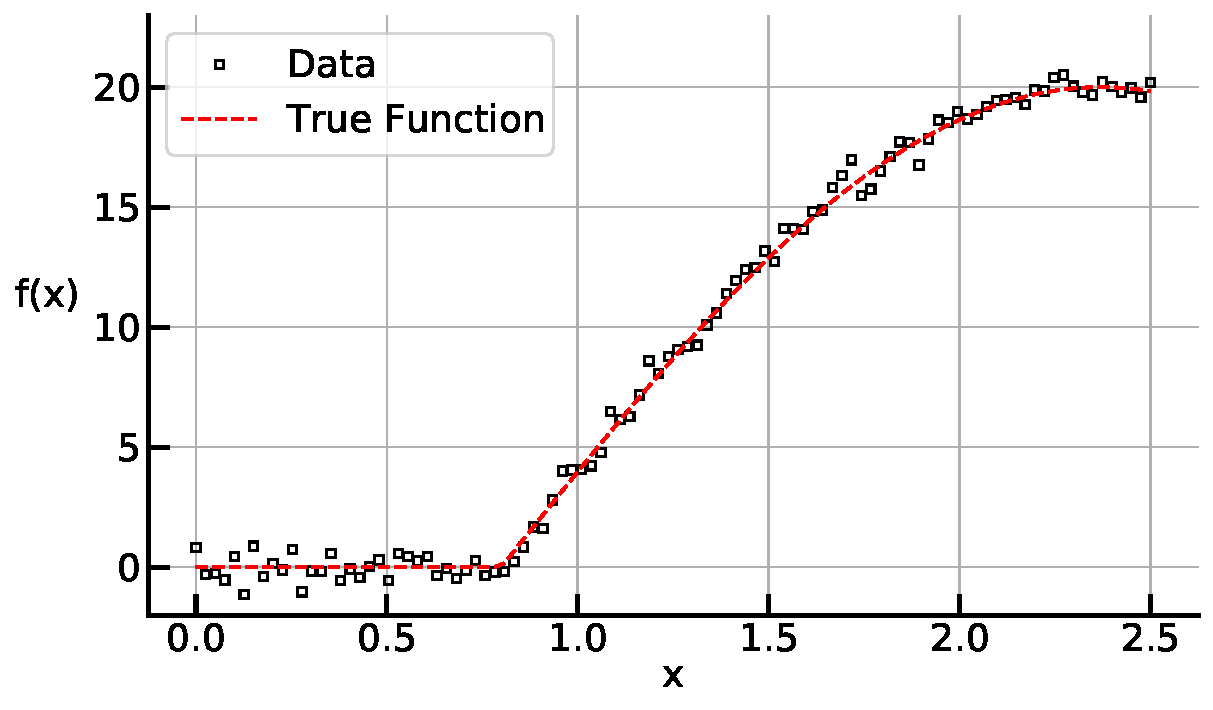
\includegraphics[width=\columnwidth]{../thesisplots/exp_inc1_data.pdf}
	\caption{Test function 1 and noisy samples}
	\label{fig:test_func_1}
\end{figure}

The second function that will be investigated is given by

\begin{equation} \label{eq:test_func_2}
	f(x) = \begin{cases}
					2\exp \big(-\frac{(x-0.5)^2}{0.05} \big) + 3x  &,\text{if} \ x \le 0.85 \\
					2\exp \big(-\frac{(0.85-0.5)^2}{0.05} \big) + 3*0.85  &,\text{else}
	       \end{cases}, \quad \text{for} \ x \in [0,1]. 	
\end{equation}

The true functions depicts a unimodal behavior and is constant for $x > 0.85$. To test the algorithm, we deliberately generate "wrong" data using the following function

\begin{equation} \label{eq:test_func_2_wrong}
	f(x) = 2\exp \big(-\frac{(x-0.5)^2}{0.05} \big) + 3x  \quad \text{for} \ x \in [0, 1]. 
\end{equation}

An example of the true function \ref{eq:test_func_2} as well as noisy samples from function \ref{eq:test_func_2_wrong} are given in Figure \ref{fig:test_func_2}.

\begin{figure}[h]
	\centering
	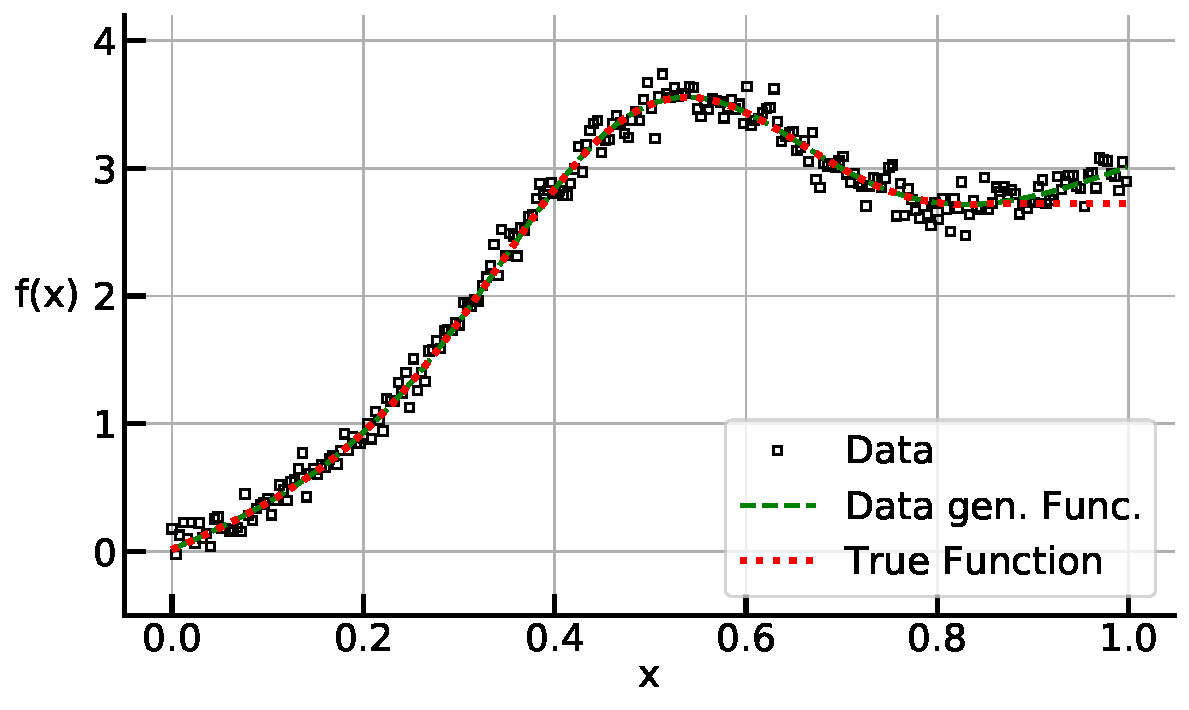
\includegraphics[width=\columnwidth]{../thesisplots/exp_peak_data.pdf}
	\caption{Test function 2 and noisy samples}
	\label{fig:test_func_2}
\end{figure}

\section{Experiments}

\subsection{Exp. 1.1: Static Function Approx. using a priori Knowledge on Function \ref{eq:test_func_1}} \label{subsec:exp11}

For the experiment using Function \ref{eq:test_func_1} in (\ref{eq:test_func_1}), the data set consists of 100 points. We use $k=35$ as number of splines. The smoothing parameter $\lambda_s$ is optimized using cross-validation given in Chapter \emph{CrossValidation}. The parameter $\lambda_c$ regulating the influence of the constraint is set to the 1000-fold of the smoothing parameter $\lambda_s$. The resulting constrained fit, and for comparison, the unconstrained fit using the optimal smoothing parameter $\lambda_s = 2.3714$ are shown in Figure \ref{fig:test_func_1_fit}.

\begin{figure}[H]
	\centering
	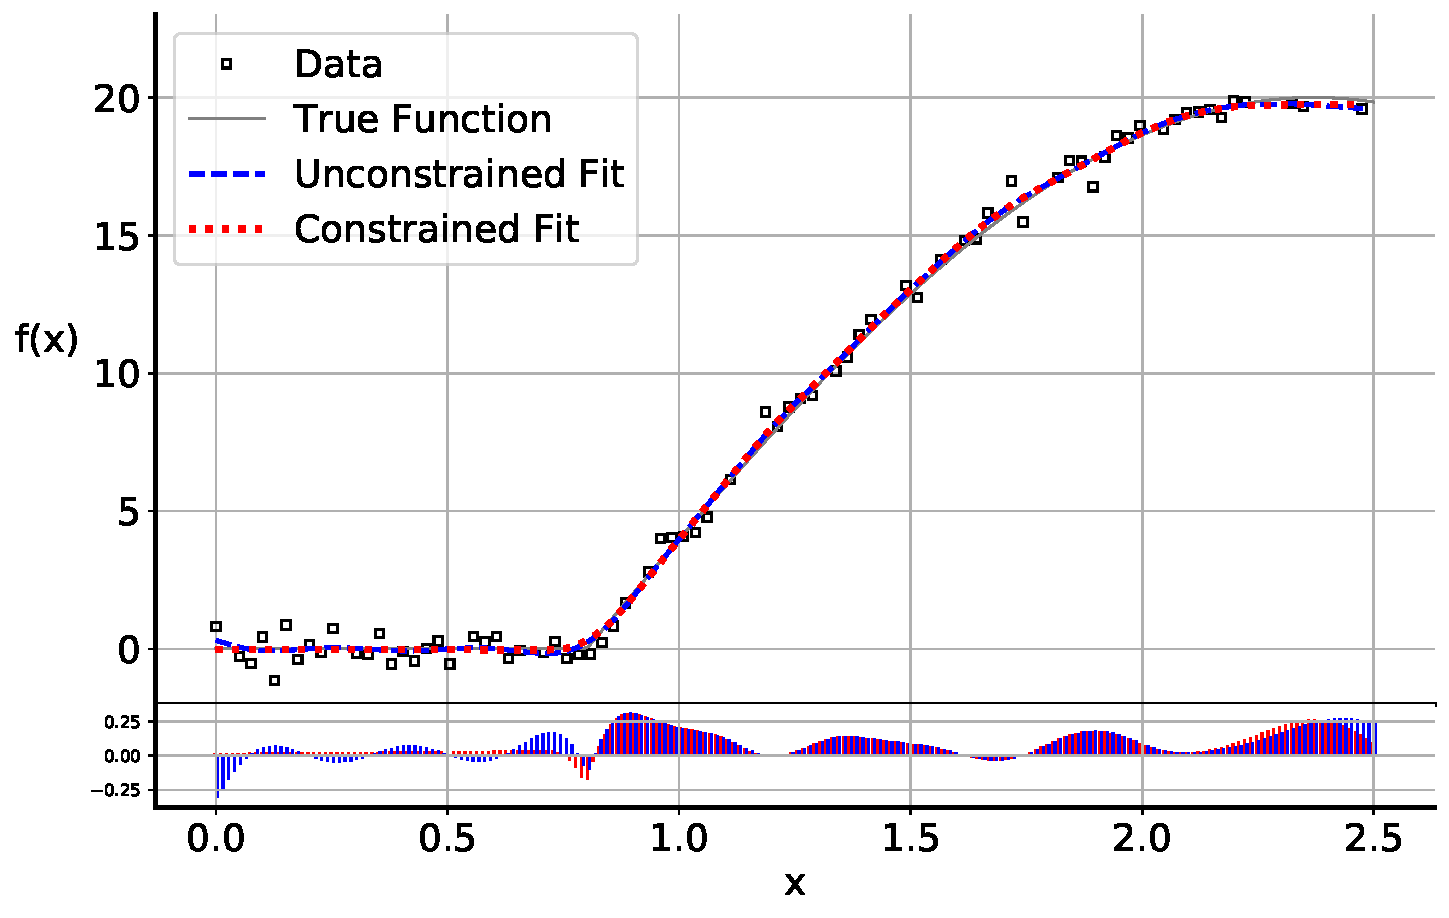
\includegraphics[width=\columnwidth]{../thesisplots/exp_inc1_fit.pdf}
	\caption{Constr. fit, unconstr. fit and residuals (lower plot) for function 1}
	\label{fig:test_func_1_fit}
\end{figure}

The red line follows the a priori knowledge of increasing behavior better than the blue, unconstrained line. Especially in the constant area, e.g. $x \in  [0, 0.45]$, the constraint improves the static function approximation and lowers the residual as seen in the lower part of Figure \ref{fig:test_func_1_fit}. In the area of increasing behavior, the two fits are almost identical since the constraint is inactive. The mean squared errors MSE on train and test set as well as the AIC value are given in Table \ref{tab:metrics_1-1}. The mean squared errors for the train and test set are of similar magnitude. Therefore, we can conclude that no overfitting is present. The AIC value for the constrained fit, as well as the MSEs, are fit are lower that the one for the unconstrained fit. 

\begin{table}[h]
	\centering
	\begin{tabular}{|l|l|l|l|}
		\hline
		\textbf{Model} & \textbf{$\text{MSE}_{train}$} & \textbf{$\text{MSE}_{test}$}  & \textbf{AIC} \\ \hline \toprule
		Unconstraint   & $4.913 * 10^{-4}$  & $6.2156 * 10^{-4}$ & -85.77       \\ \hline
		Constraint     & $3.205* 10^{-4}$   & $2.6096 * 10^{-4}$ & -157.5       \\ \hline \bottomrule
	\end{tabular}
	\caption{MSEs and AIC for Exp. 1.1}
	\label{tab:metrics_1-1}
\end{table}

The use of a priori domain knowledge through user-defined constraints therefore improves the fitting quality quantitatively, see Table \ref{tab:metrics_1-1}, as well as qualitatively, see Figure \ref{fig:test_func_1_fit}.

%%
%As with likelihood, the absolute value of AIC is largely meaningless (being determined by the arbitrary constant). As this constant depends on the data, AIC can be used to compare models fitted on identical samples. The best model from the set of plausible models being considered is therefore the one with the smallest AIC value (the least information loss relative to the true model).

%A common misconception is to think that the goal is to minimize the absolute value of AIC, but the arbitraty constant can (depending on data and model) produce negative values. Negative AIC indicates less information loss than a positive AIC and therefore a better model.

%Source: Baguley, Thomas. Serious stats: A guide to advanced statistics for the behavioral sciences. Palgrave Macmillan, 2012. (page 402)


\subsection{Exp. 1.2: Static Function Approx. using a priori Knowledge on Function \ref{eq:test_func_2}} \label{subsec:exp12}

For the test using Function \ref{eq:test_func_2} in (\ref{eq:test_func_2}), the data set consists of 500 points. There are two possibilities to include the a priori knowledge of a unimodal behavior. First we can use the peak constraint matrix given in Chapter \emph{Unimodality Constraint}. On the other hand, we can use the concavity constraint, since concave functions are likely to have a peak when the data shows a peak. 

We examine both possibilities in Figure \ref{fig:test_func_2_fit}. For each fit, we used $k=35$ as number of splines and the smoothing parameter $\lambda_s=510.87$ was again optimized using cross-validation. The constraint parameter $\lambda_c$ was set to $5109$.

\begin{figure}[H]
	\centering
	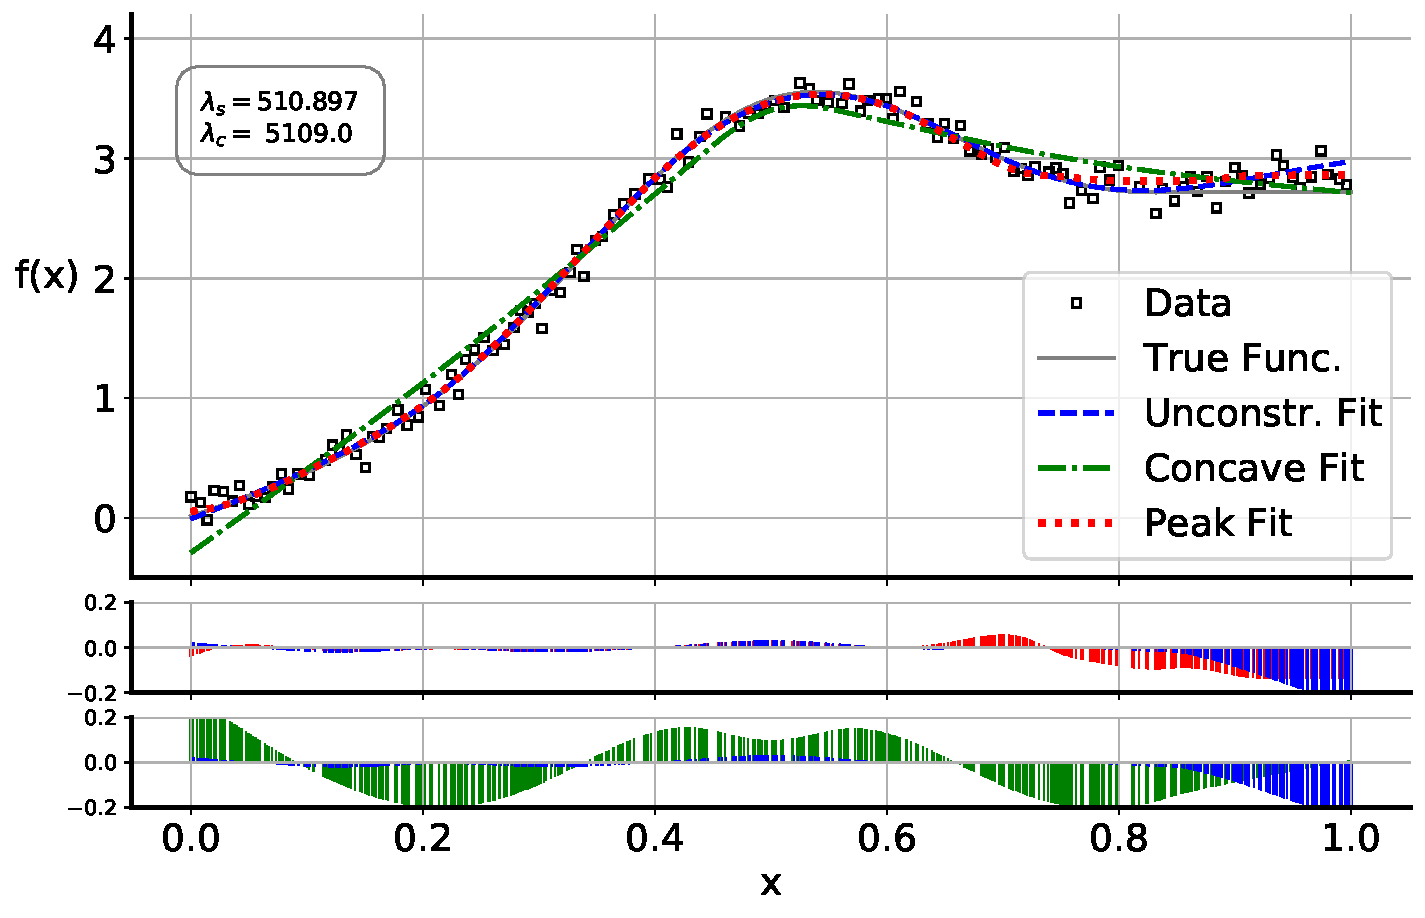
\includegraphics[width=\columnwidth]{../thesisplots/exp_peak_fit.pdf}
	\caption{Constr. fit, unconstr. fit and residuals (lower plots) for function 2}
	\label{fig:test_func_2_fit}
\end{figure}
 
The estimate for the concave constraint shows the desired peak behavior, and is more smooth than the peak constraint estimate. This smoothness leads to changes in the sign of the residuals compared to the unconstrained fit as seen in the lower part of Figure \ref{fig:test_func_2_fit}. The peak constraint identifies the peak correctly and produces a sufficiently smooth fit with low residual. Especially for $x >0.8$, i.e. the region where the data is on purpose "wrong", the estimate of the peak constrained fit is almost constant while the concave constrained fit is decreasing. 

The mean squared errors and the ACI value are given in the Table \ref{tab:metrics_1-2}. They show that the concave constraint fit is has higher MSE on train and test set, as well as a higher AIC value. The more accurate fit are therefore produced by the peak constraint. The AIC value implies to use the unconstrained model, since it possesses the lowest value. Nevertheless, as seen in Figure \ref{fig:test_func_2_fit}, it violates the user-defined constraint for larger $x$. Therefore, the peak constrained model is the best model with respect to the a priori knowledge. 

\begin{table}[h]
	\centering
	\begin{tabular}{|l|l|l|l|}
		\hline
		\textbf{Model} & \textbf{$\text{MSE}_{train}$} & \textbf{$\text{MSE}_{test}$}  & \textbf{AIC} \\ \hline \toprule
		Unconstraint        & $0.3839 * 10^{-3}$   & $5.6641 * 10^{-2}$ & -705.1       \\ \hline
		Concave Constraint  & $1.7563 * 10^{-3}$   & $5.9008 * 10^{-2}$ & -481.4       \\ \hline 
		Peak Constraint     & $0.3400 * 10^{-3}$   & $5.7031 * 10^{-2}$ & -696.2       \\ \hline \bottomrule
	\end{tabular}
	\caption{MSEs and AIC for Exp. 1.1}
	\label{tab:metrics_1-2}
\end{table}

\subsection{Constraint vs. Noise} \label{subsec:constraint-vs-noise}

In this section, we investigate the effect of different noise levels as well as noise types on the fitting process. In the first part, various levels of Gaussian noise are applied to Function \ref{eq:test_func_2}. In the second part, we will use different colors of noise acting on Function \ref{eq:test_func_1}. For both examples we use $k=35$ splines and optimize the smoothing parameter $\lambda_s$ using cross-validation. 

\subsubsection{Exp. 2: Different Noise Levels}

Gaussian noise is characterized by the following two parameters:
\begin{itemize}
	\item Location: The mean value $\mu$ of the Gaussian distribution.
	\item Scale: The variance value $\sigma^2$ of the Gaussian distribution.
\end{itemize}

We set the location equal to zero and vary the scale value. The effect of the noise on the fitting procedure is shown in Figure \ref{fig:fit_noise_levels}. The chosen noise levels are $\sigma^2 = \{0.01, 0.05, 0.1\}$.

For these values of $\sigma^2$, the correspond optimized smoothing parameters are $\lambda_{0.01} = 320$, $\lambda_{0.05} = 1892$ and $\lambda_{0.1} = 1516$. The constraint parameter $\lambda_c$ was set to $\lambda_c = 1000 \lambda_s$. 

\begin{figure}[H]
	\centering
	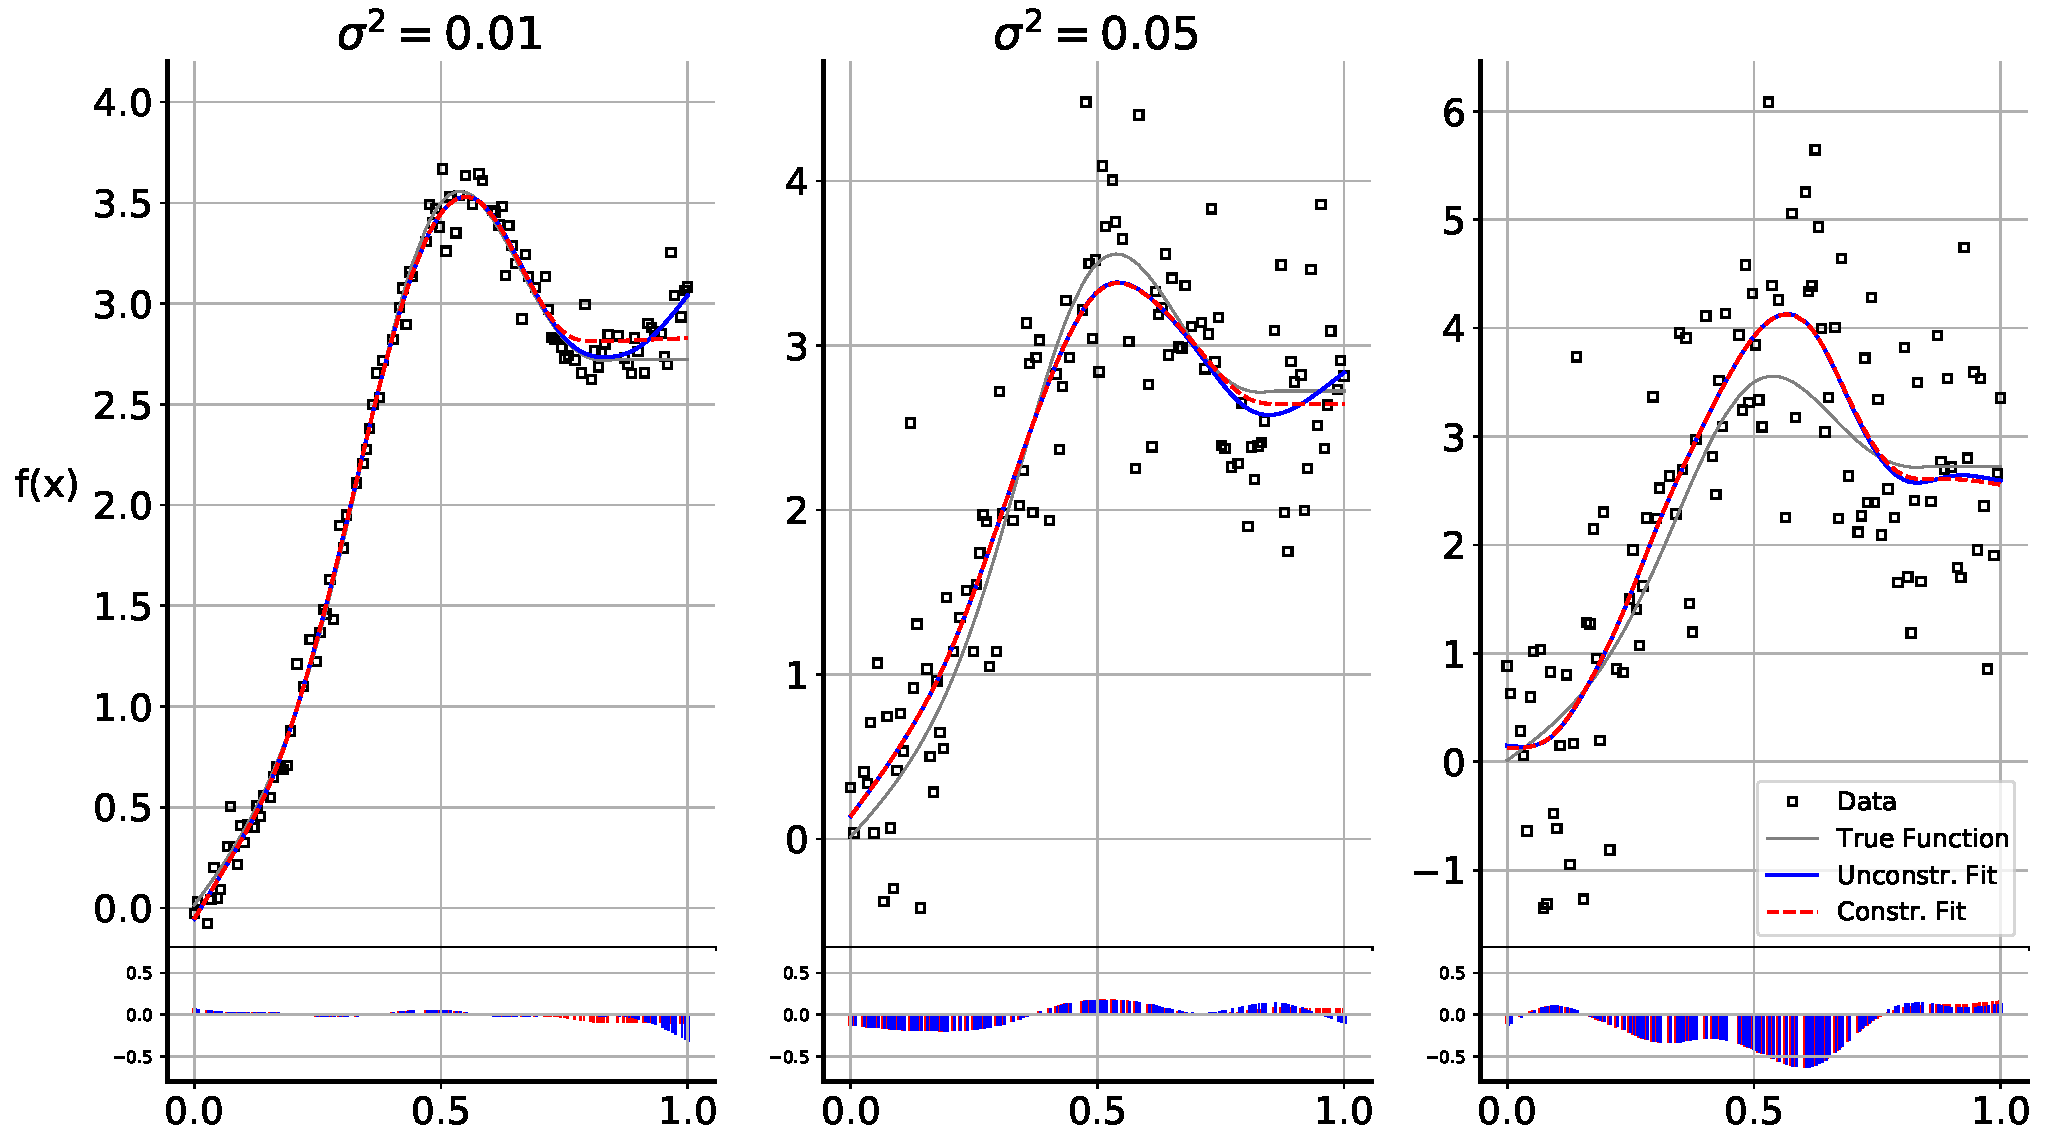
\includegraphics[width=\columnwidth]{../thesisplots/exp_noise_levels.pdf}
	\caption{Constr. fit, unconstr. fit and residuals for various noise levels}
	\label{fig:fit_noise_levels}
\end{figure}

The left plot shows the fit for $\sigma^2 = 0.01$. The noise level is moderate, which leads to a smooth and satisfying fit except for large $x$ where the fit does not meet the constant function level. The peak constraint is well satisfied. 

The noise level in the middle plot is already high. The unconstrained fit is nevertheless smooth, but it underestimates the peak and violates the constraint for $x > 0.8$. The constrained fit holds the peak constraint and produces a satisfying fit despite the high noise level.

For the right plot and $\sigma^2=0.1$, both constrained and unconstrained fit are smooth but overestimate the fit especially in the peak region. The noise level is very high and the fits must be used carefully. 

Structured additive regression using a priori domain knowledge can be used to estimate smooth, constraint functions even if the measurement noise is quite high, see the middle plot in Figure \ref{fig:fit_noise_levels}. For very high noise levels, the constraint can also be used to enforce a priori known behavior.  

\subsubsection{Exp. 3: Different Noise Colors}

We investigate the effect of different noise color on the function fitting process. The tested colors are the following power-law noise types:

\begin{itemize}
	\item  White Noise
	\item Pink Noise
	\item Brownian Noise
\end{itemize}

The unconstrained as well as the increasing constrained fit for all noise colors are shown in Figure \ref{fig:fit_noise_colors}.

\begin{figure}[H]
	\centering
	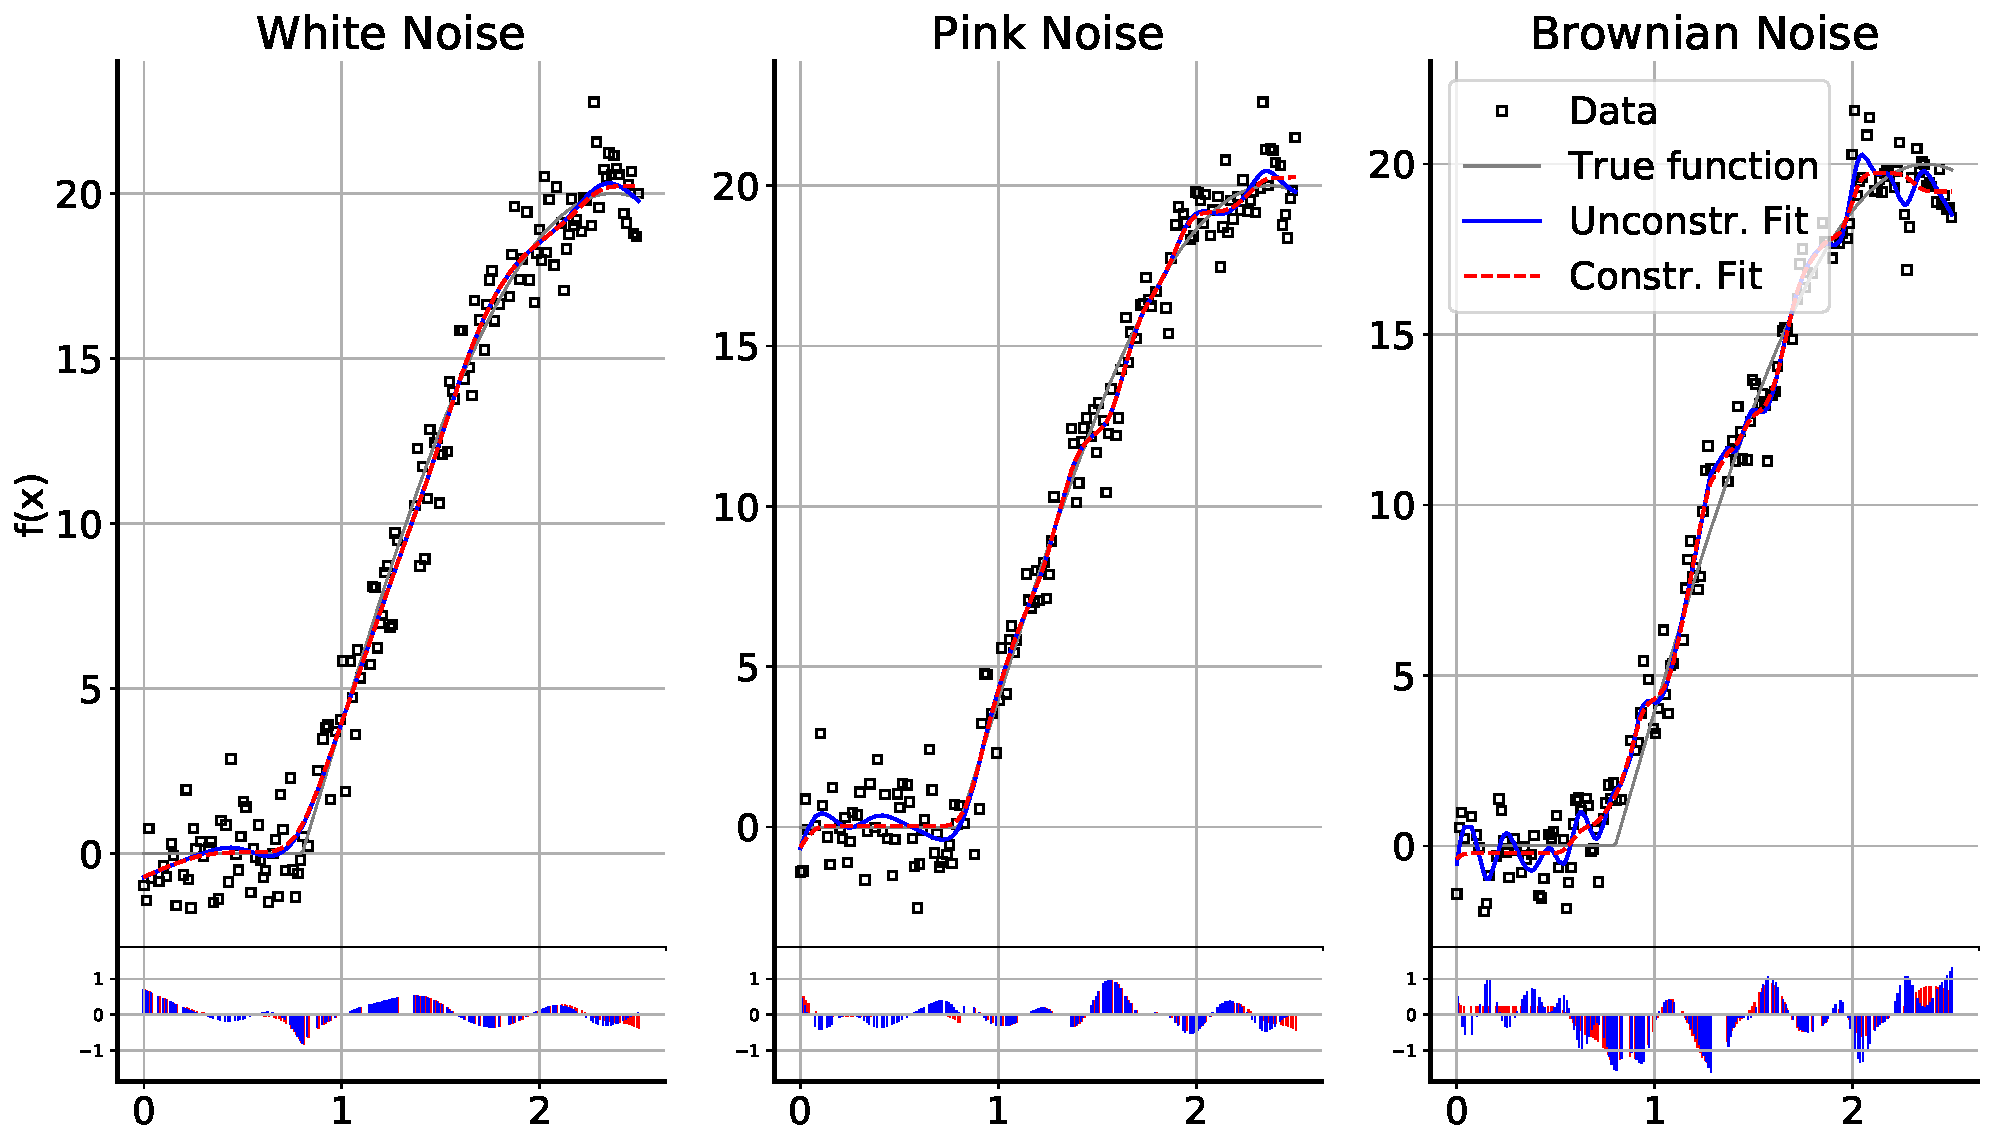
\includegraphics[width=\columnwidth]{../thesisplots/exp_noise_colors.pdf}
	\caption{Constr. and unconstr. fit and residuals for noise colors}
	\label{fig:fit_noise_colors}
\end{figure}

For the white noise data in the left plot, the increasing constraint produces a good fit according to the constraint and the residual except for low $x < 0.1$. The optimized smoothing parameter for the unconstrained fit was given by $\lambda_s = 132.07$ and the constraint parameter was set to $\lambda_c = 1320$. The fit recovers the true function quite well. 

For the pink noise data in the middle plot, the constraint helps regularizing the fit. The constant function part was fit very well, as seen in the residual part in Figure \ref{fig:fit_noise_colors}. The increasing part of the function, i.e. $f(x)$ for $x \ge 0.45$,  was fit well. The smoothing parameter was optimized using cross-validation and set to $\lambda_s = 20.67$. The constraint parameter was set to $\lambda_c = 2067$. 

For the brownian noise data in the right plot, the increasing part of the function was recovered well. The increasing constraint is hold quite well. Nevertheless, the brownian noise leads to step function like artifacts in the estimate for the constrained fit. The optimized smoothing parameter used was $\lambda_s = 0.4209$ and the constraint parameter was set to $\lambda_c = 4208$.

\subsection{Well-distributed vs. Skewed Data and Knot Placement} \label{subsec:skewed-data}
We will now investigate the effect of irregular data distributions on the fitting process. The main question is if any knot placement type is superior to the other. We therefore examine input data $x^{(i)}$ for $i = 1, \dots, n$ generated on a grid vs. data generated from a beta distribution given by

\begin{align}
	f(x) = \frac{1}{B(a, b))} x^{a-1} (1-x)^{b-1} 
\end{align}
with
\begin{align}
	B(a,b) = \frac{\Gamma(a)\Gamma(b)}{\Gamma(a+b)} = \int_0^1 u^{a-1} (1-u)^{b-1} du
\end{align}


for different values of the parameters $a$ and $b$. We will investigate the effect of the knot placement, which can either be equidistant knot placement or quantile based knot placement, using this data. We again use noisy samples from function \ref{eq:test_func_2} and $k=35$ as number of splines. The smoothing parameters were optimized using cross-validation. The constraint parameters were set to the $1000-\text{fold}$ of $\lambda_s$ or adjusted by hand.

\subsubsection{Exp. 4: Equidistant vs. Quantile Based Knot Placement for Grid Data}

We will use 250 noisy samples from Function \ref{eq:test_func_2} in (\ref{eq:test_func_2}) generated from a equidistant sequence of $x$. The smoothing parameters for the equidistant knot placement fit and for the quantile based knot placement fit were optimized using cross-validation and set to $\lambda_{s,equidistant} = 17.7828$ and $\lambda_{s, quantile} = 0.0056$. The constraint parameter for the peak constraint was set to $\lambda_c = 4000$ for both fits. The resulting fits are shown in Figure \ref{fig:fit_grid_250}.

\begin{figure}[H]
	\centering
	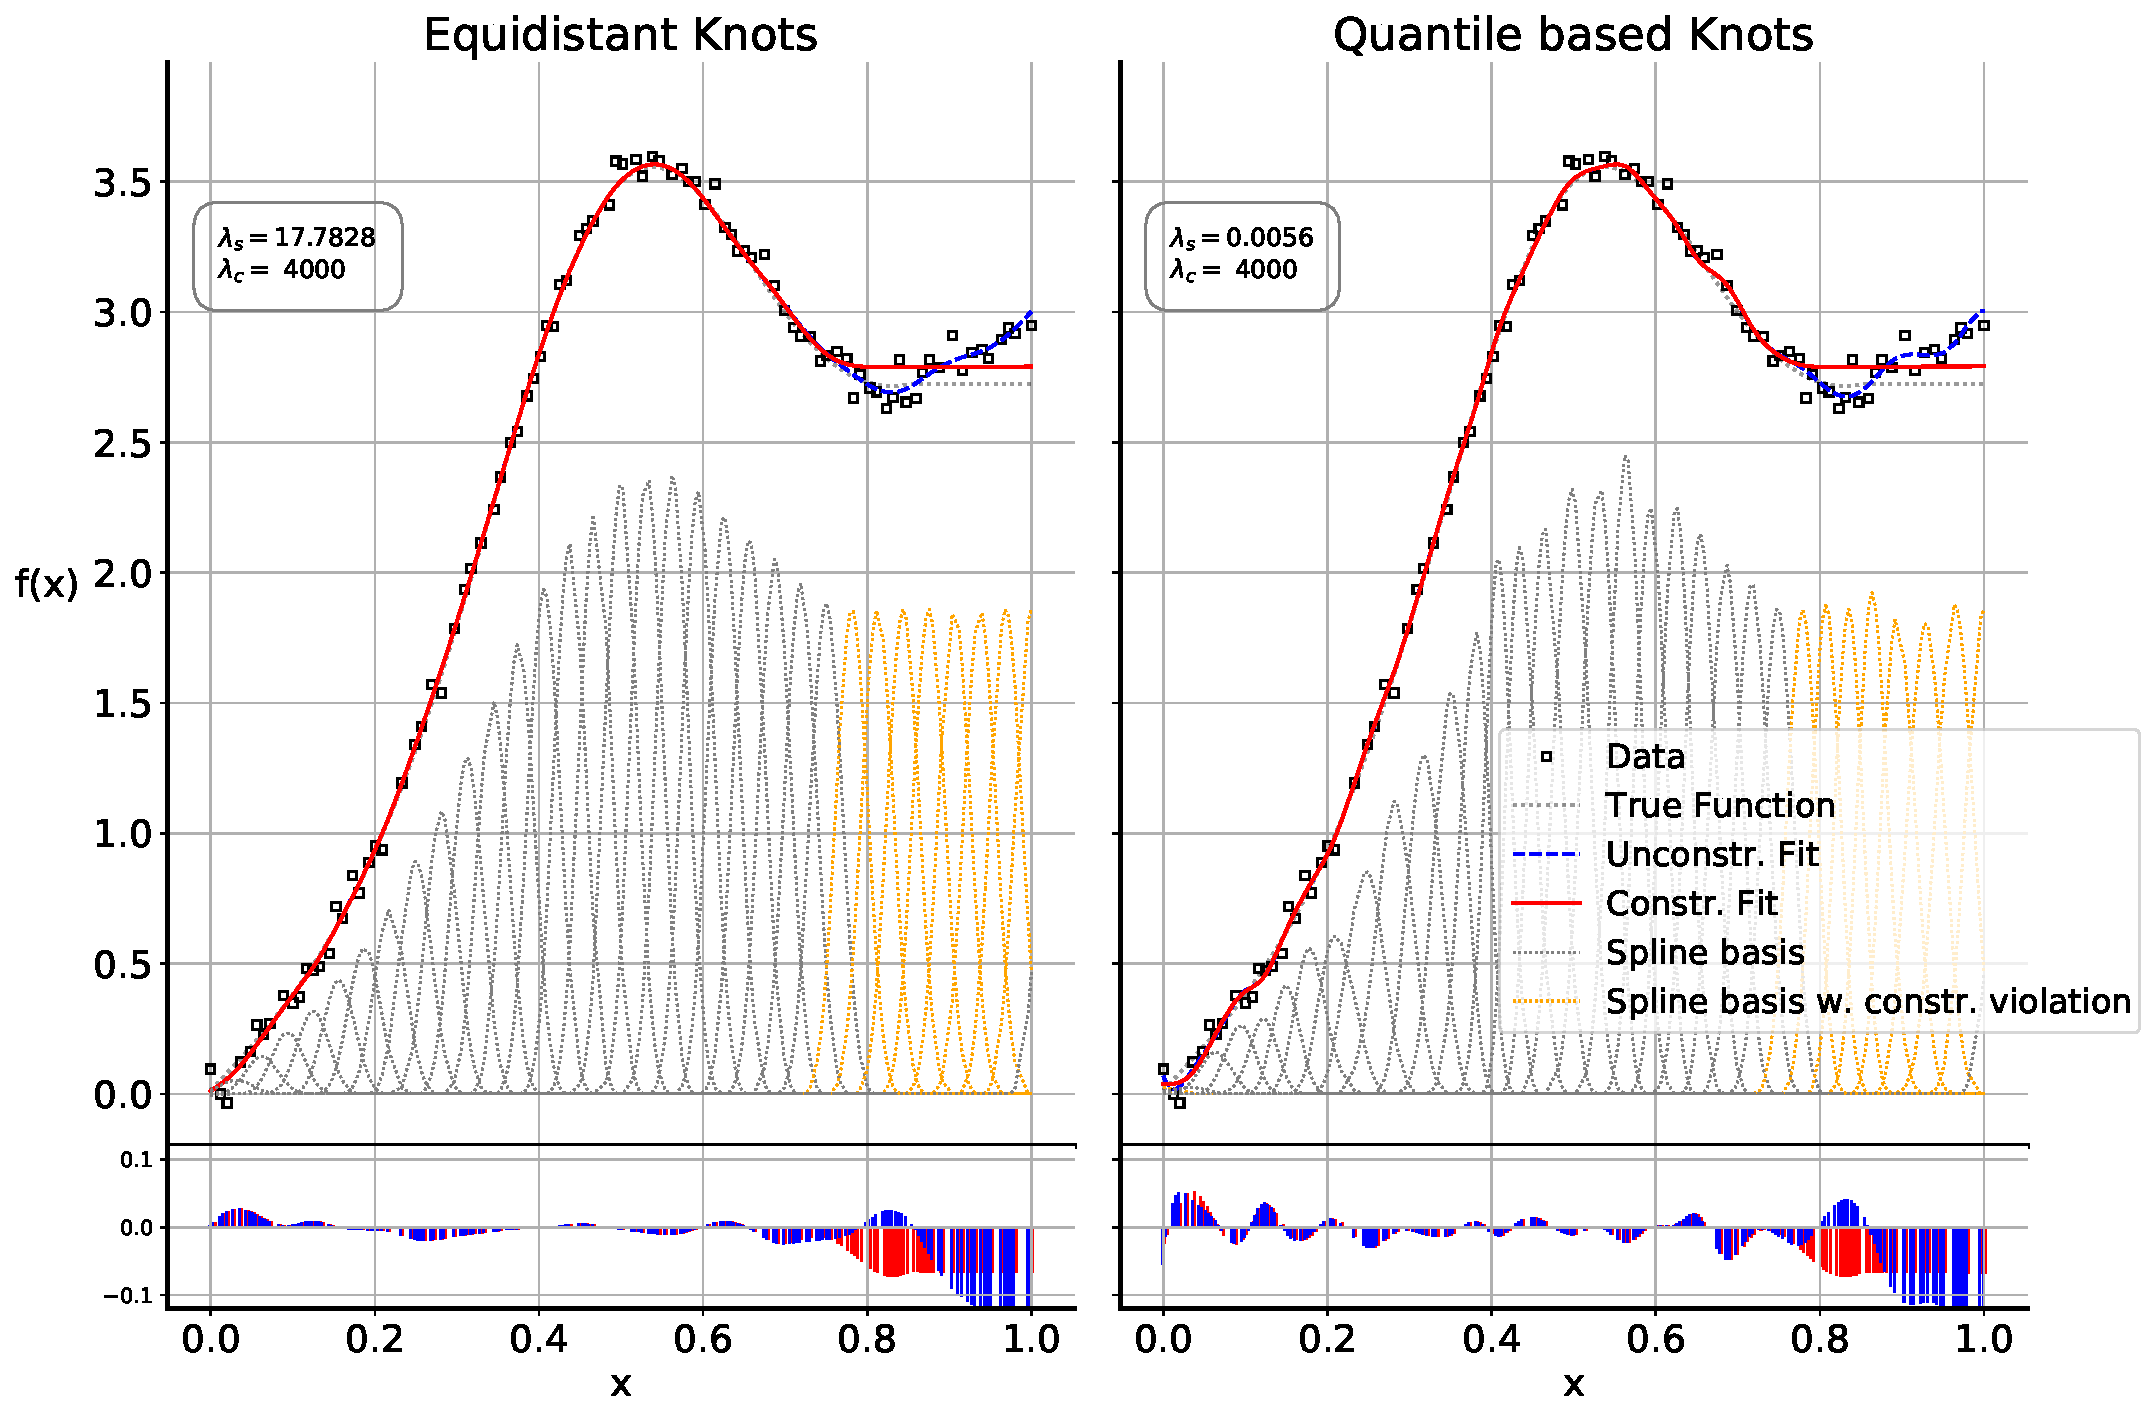
\includegraphics[width=\columnwidth]{../thesisplots/exp_grid/exp_grid_ndata_250_rseed_1.pdf}
	\caption{Constr. and unconstr. fit and residuals for grid data}
	\label{fig:fit_grid_250}
\end{figure}

Figure \ref{fig:fit_grid_250} shows not much difference between the fits for the knot placement types. The peak constraint is hold by both quite well. The residuals for  equidistant knot placement are overall lower. The fit using equidistant knot placement is more smooth, since its optimal smoothing parameter is higher compared to the quantile based knot placement estimate. This can also be seen in the residual part of Figure \ref{fig:fit_grid_250}. 

The mean squared errors and AIC values are given in Table \ref{tab:metrics_4}. In this table, "E" stands for equidistant knot placement and "Q" stands for quantile based knot placement. The equidistant model has lower MSEs for train and test set, as well as a lower AIC value, compared to the quantile model for both the constrained and unconstrained fit. 

\begin{table}[h]
	\centering
	\begin{tabular}{|l|l|l|l|}
		\hline
		\textbf{Model} & \textbf{$\text{MSE}_{train}$} & \textbf{$\text{MSE}_{test}$}  & \textbf{AIC} \\ \hline \toprule
		Unconstraint + E  & $2.72 * 10^{-3}$  & $4.43 * 10^{-3}$ & -280.7       \\ \hline
		Unconstraint + Q  & $3.02 * 10^{-3}$  & $5.20 * 10^{-3}$ & -208.2       \\ \hline
		Constraint + E    & $1.07 * 10^{-3}$  & $1.11 * 10^{-3}$ & -379.9       \\ \hline
		Constraint + Q    & $1.24 * 10^{-3}$  & $1.31 * 10^{-3}$ & -334.4       \\ \hline \bottomrule
	\end{tabular}
	\caption{MSEs and AIC for Exp. 4}
	\label{tab:metrics_4}
\end{table}


\subsubsection{Exp. 5.1: Equidistant vs. Quantile Based Knot Placement for Left Skewed Data} \label{subsubsec:left_skew}

We will now investigate the effect of non-regular data distributions for Function \ref{eq:test_func_2} in (\ref{eq:test_func_2}) given by a beta distribution with $a = 1$ and $b = 3$. Therefore the situation is that we have many data points in the increasing part for $x \le 0.4$ and little points for the constant function part at $x > 0.8$. The fits for equidistant and quantile based knot placement can be seen in Figure \ref{fig:fit_left_skew_250}. 

\begin{figure}[H]
	\centering
	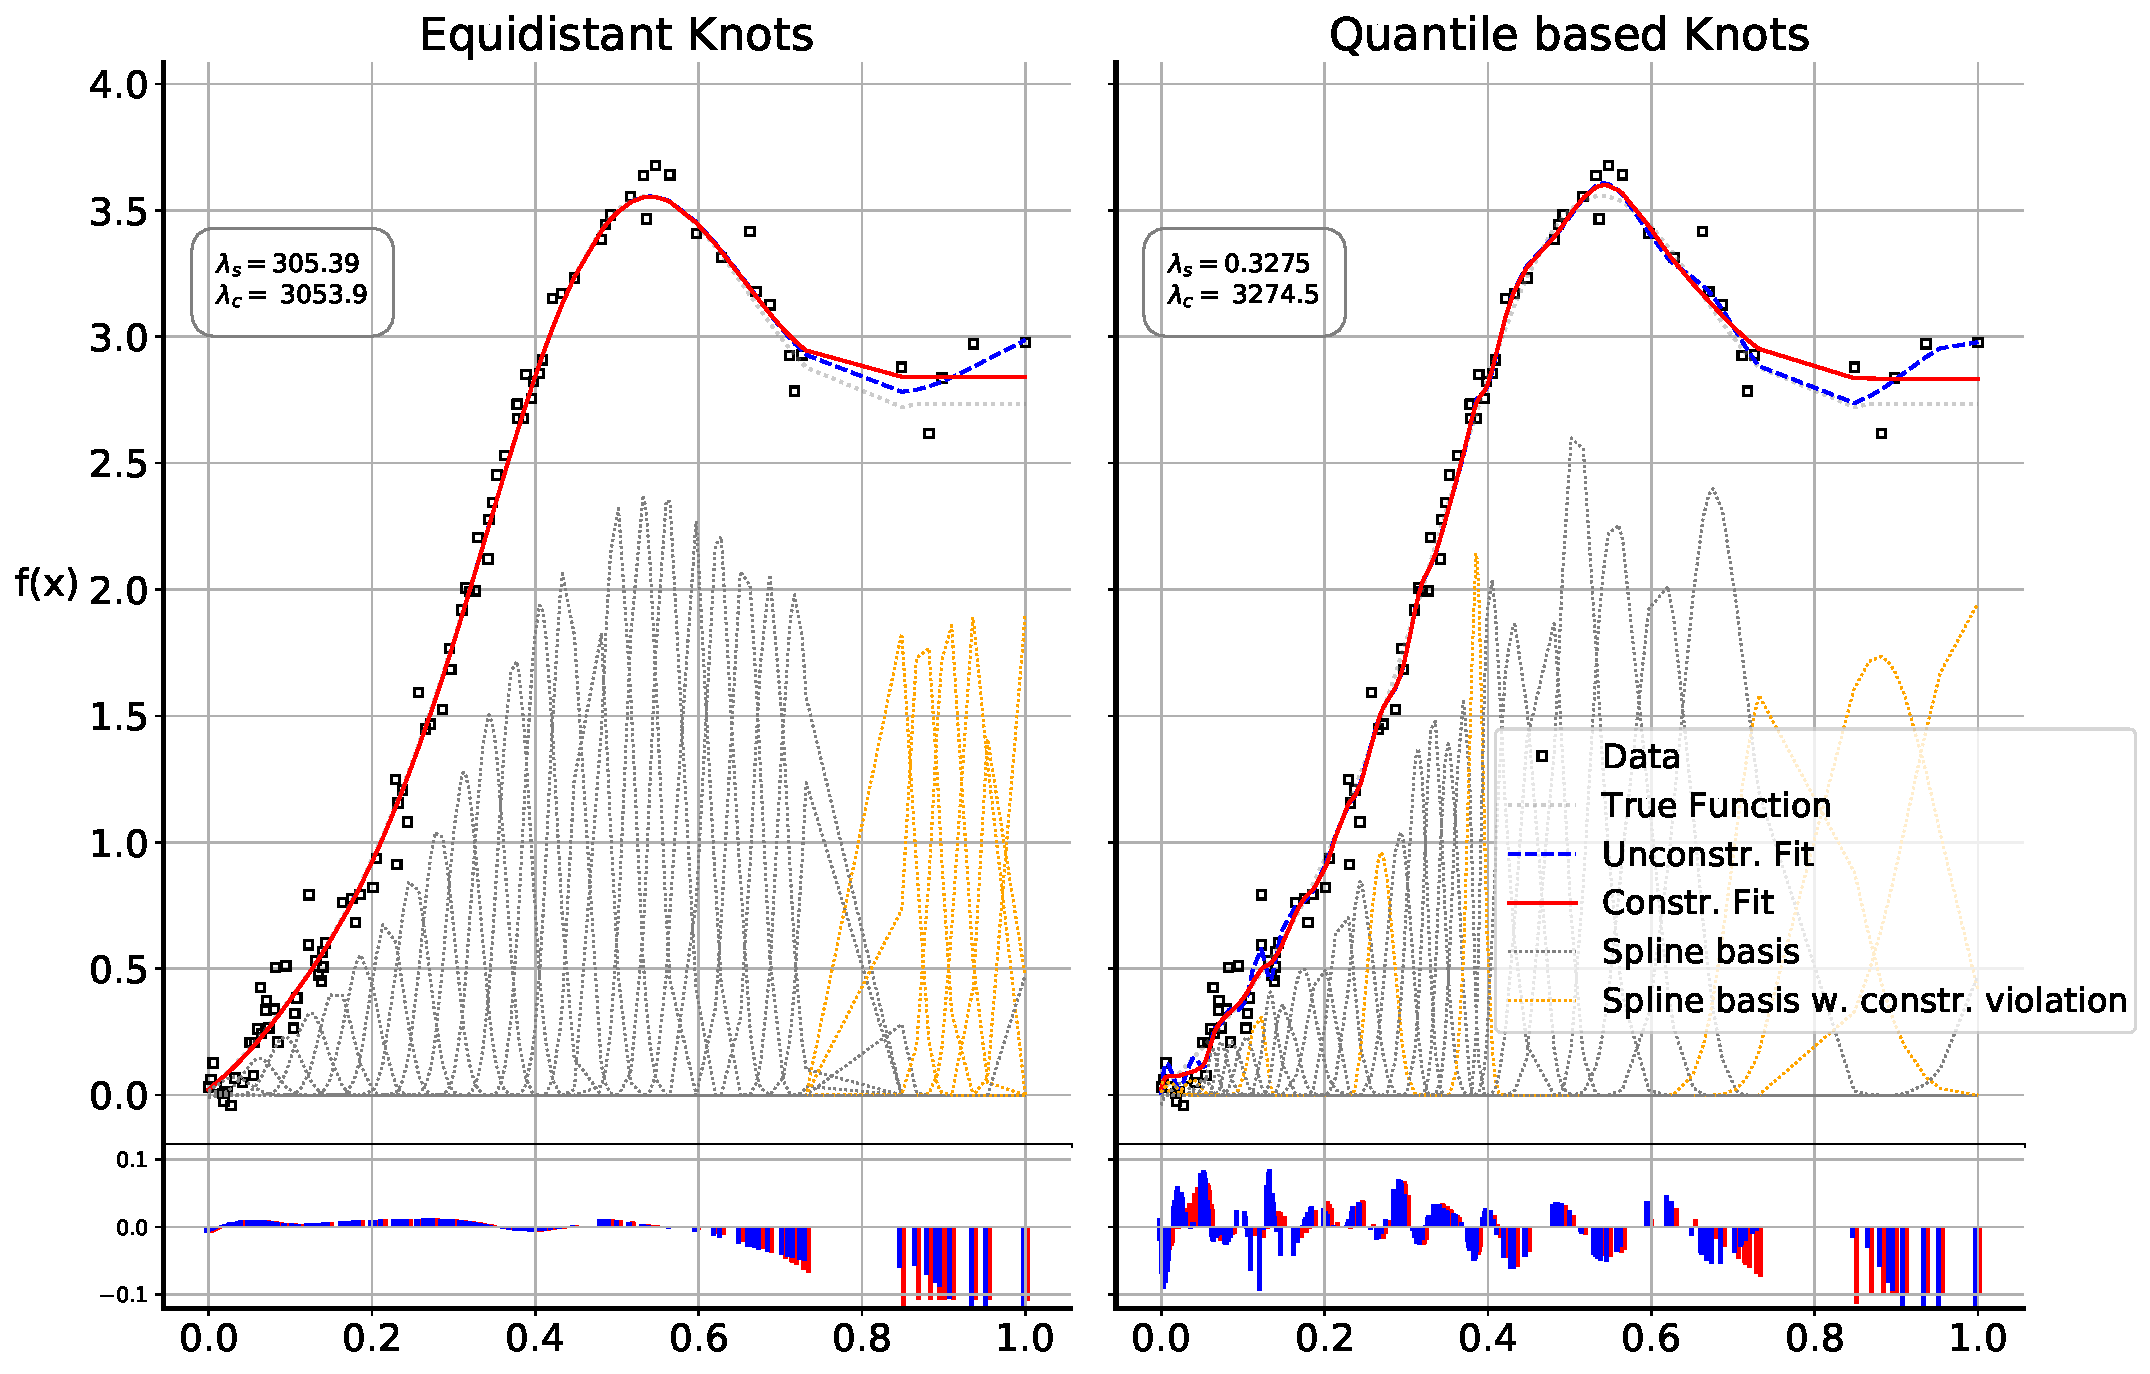
\includegraphics[width=\columnwidth]{../thesisplots/exp_beta/exp_left_skewed_data_ndata_250_rseed_1.pdf}
	\caption{Constr. and unconstr. fit and residuals for left skewed data}
	\label{fig:fit_left_skew_250}
\end{figure}

The smoothing parameters were set to $\lambda_{s, equidistant} = 305.39$ for equidistant knot placement and $\lambda_{s, quantile} = 0.3275$ for quantile based knot placement. This low optimal smoothing parameter leads to a wiggly estimate for the quantile based knot placement fit compared the the smooth estimate for equidistant knot placement. This can also be seen in the residual part of Figure \ref{fig:fit_left_skew_250}. The constraint parameters were set to $\lambda_{c, equidistant} = 3053.9$ and $\lambda_{c, quantile} = 3274.5$. The constraint is hold for both knot types. Especially for large $x > 0.9$ we see an improvement in the residual as well as the qualitative behavior for the constraint fits. 

The mean squared errors on training and test set as well as the AIC values are given in Table \ref{tab:metrics_51}. Again, "E" stands for equidistant knot placement and "Q" stands for quantile based knot placement. The constraint, equidistant model produces the lowest $\text{MSE}_{train}$. The MSEs on the test set are of the same magnitude as for the train set, indication that there is no overfitting present. The lowest AIC values is present for the unconstraint equidistant model. Nevertheless, the constraint violation of this model is clearly visible in Figure \ref{fig:fit_left_skew_250}.

\begin{table}[H]
	\centering
	\begin{tabular}{|l|l|l|l|}
		\hline
		\textbf{Model} & \textbf{$\text{MSE}_{train}$} & \textbf{$\text{MSE}_{test}$}  & \textbf{AIC} \\ \hline \toprule
		Unconstraint + E  & $0.98 * 10^{-3}$  & $0.74 * 10^{-3}$ & -421.3       \\ \hline
		Unconstraint + Q  & $2.46 * 10^{-3}$  & $2.08 * 10^{-3}$ & -288.2       \\ \hline
		Constraint + E    & $0.78 * 10^{-3}$  & $1.09 * 10^{-3}$ & -400.2       \\ \hline
		Constraint + Q    & $1.41 * 10^{-3}$  & $1.78 * 10^{-3}$ & -311.5      \\ \hline \bottomrule
	\end{tabular}
	\caption{MSEs and AIC for Exp. 5.1}
	\label{tab:metrics_51}
\end{table}


\subsubsection{Exp. 5.2: Equidistant vs. Quantile Based Knot Placement for Middle Skewed Data}

We will now investigate the effect of non-regular data distributions for Function \ref{eq:test_func_2} in (\ref{eq:test_func_2}) given by a beta distribution with $a = 3$ and $b = 3$. Therefore the situation is that we have many data points in the peak part for $x \in [0.3, 0.7]$ and less points for the constant function part at $x > 0.7$ and the increasing part at $x < 0.3$. The fits for equidistant and quantile based knot placement can be seen in Figure \ref{fig:fit_middle_skew_250}. 

\begin{figure}[H]
	\centering
	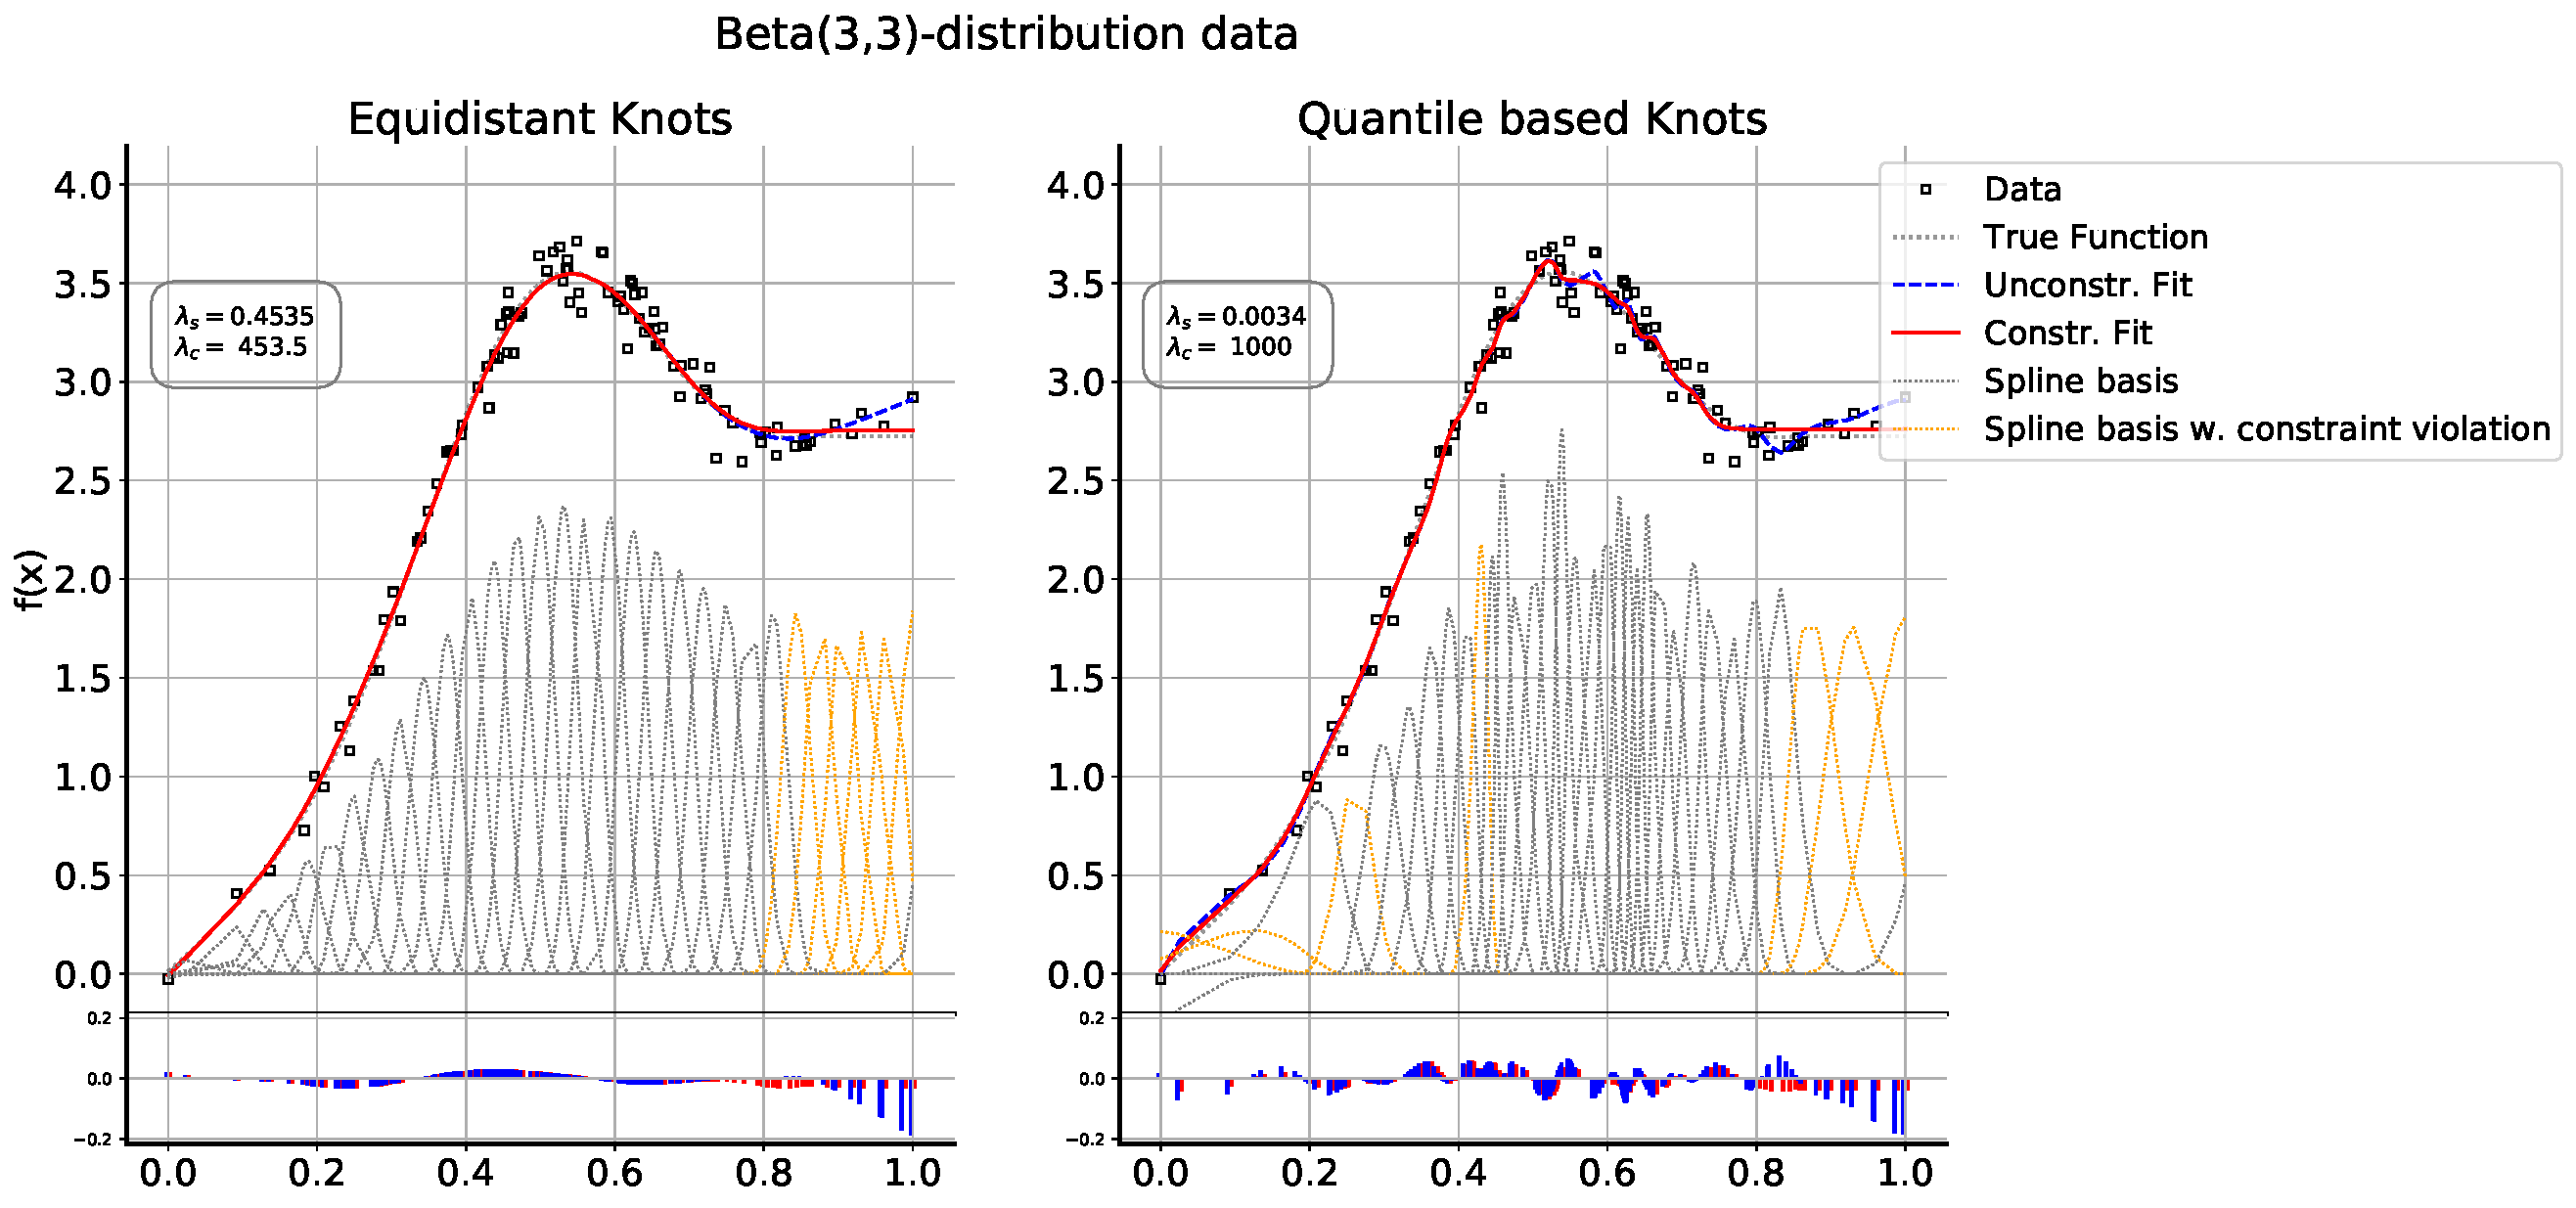
\includegraphics[width=\columnwidth]{../thesisplots/exp_beta/exp_middle_skewed_data_ndata_250_rseed_1.pdf}
	\caption{Constr. and unconstr. fit and residuals for middle skewed data}
	\label{fig:fit_middle_skew_250}
\end{figure}

The smoothing parameters were set to $\lambda_{s, equidistant} = 422.92$ for equidistant knot placement and $\lambda_{s, quantile} = 0.0091$ for quantile based knot placement. The low optimal smoothing parameter again leads to a wiggly estimate in the peak region for the quantile based knot placement fit compared the the smooth estimate for equidistant knot placement. This can also be seen in the residual part of Figure \ref{fig:fit_middle_skew_250}. The constraint parameters were set to $\lambda_{c, equidistant} = 4229$ and $\lambda_{c, quantile} = 9111.6$. The constraint is hold for both knot types. The equidistant knot placement produces a almost optimal fit especially for the peak region. The quantile based knot placements fit is also quite good compared to the true function, but the estimate is quite wiggly.

The mean squared errors on training and test set as well as the AIC values are given in Table \ref{tab:metrics_52}. The situation is quite similar to the left skewed data experiment given in Chapter \ref{subsubsec:left_skew}. The constraint equidistant model is the overall best model producing the lowest $\text{MSE}_{train}$ and $\text{MSE}_{test}$ as well as AIC value. This coincides with the plots in Figure \ref{fig:fit_middle_skew_250}. 

\begin{table}[H]
	\centering
	\begin{tabular}{|l|l|l|l|}
		\hline
		\textbf{Model} & \textbf{$\text{MSE}_{train}$} & \textbf{$\text{MSE}_{test}$}  & \textbf{AIC} \\ \hline \toprule
		Unconstraint + E  & $0.96 * 10^{-3}$  & $0.41 * 10^{-3}$ & -459.2       \\ \hline
		Unconstraint + Q  & $2.14 * 10^{-3}$  & $1.85 * 10^{-3}$ & -273.4       \\ \hline
		Constraint + E    & $0.44 * 10^{-3}$  & $0.37 * 10^{-3}$ & -469.8       \\ \hline
		Constraint + Q    & $0.94 * 10^{-3}$  & $0.79 * 10^{-3}$ & -366.1      \\ \hline \bottomrule
	\end{tabular}
	\caption{MSEs and AIC for Exp. 5.2}
	\label{tab:metrics_52}
\end{table}


\subsubsection{Exp. 5.3: Equidistant vs. Quantile Based Knot Placement for Right Skewed Data}

We will now investigate the effect of non-regular data distributions for Function \ref{eq:test_func_2} in (\ref{eq:test_func_2}) given by a beta distribution with $a = 3$ and $b = 1$. Therefore the situation is that we have many data points in the constant part for $x > 0.7$ and less points for the increasing and peak part $x < 0.7$. The fits for equidistant and quantile based knot placement can be seen in Figure \ref{fig:fit_right_skew_250}. 

\begin{figure}[H]
	\centering
	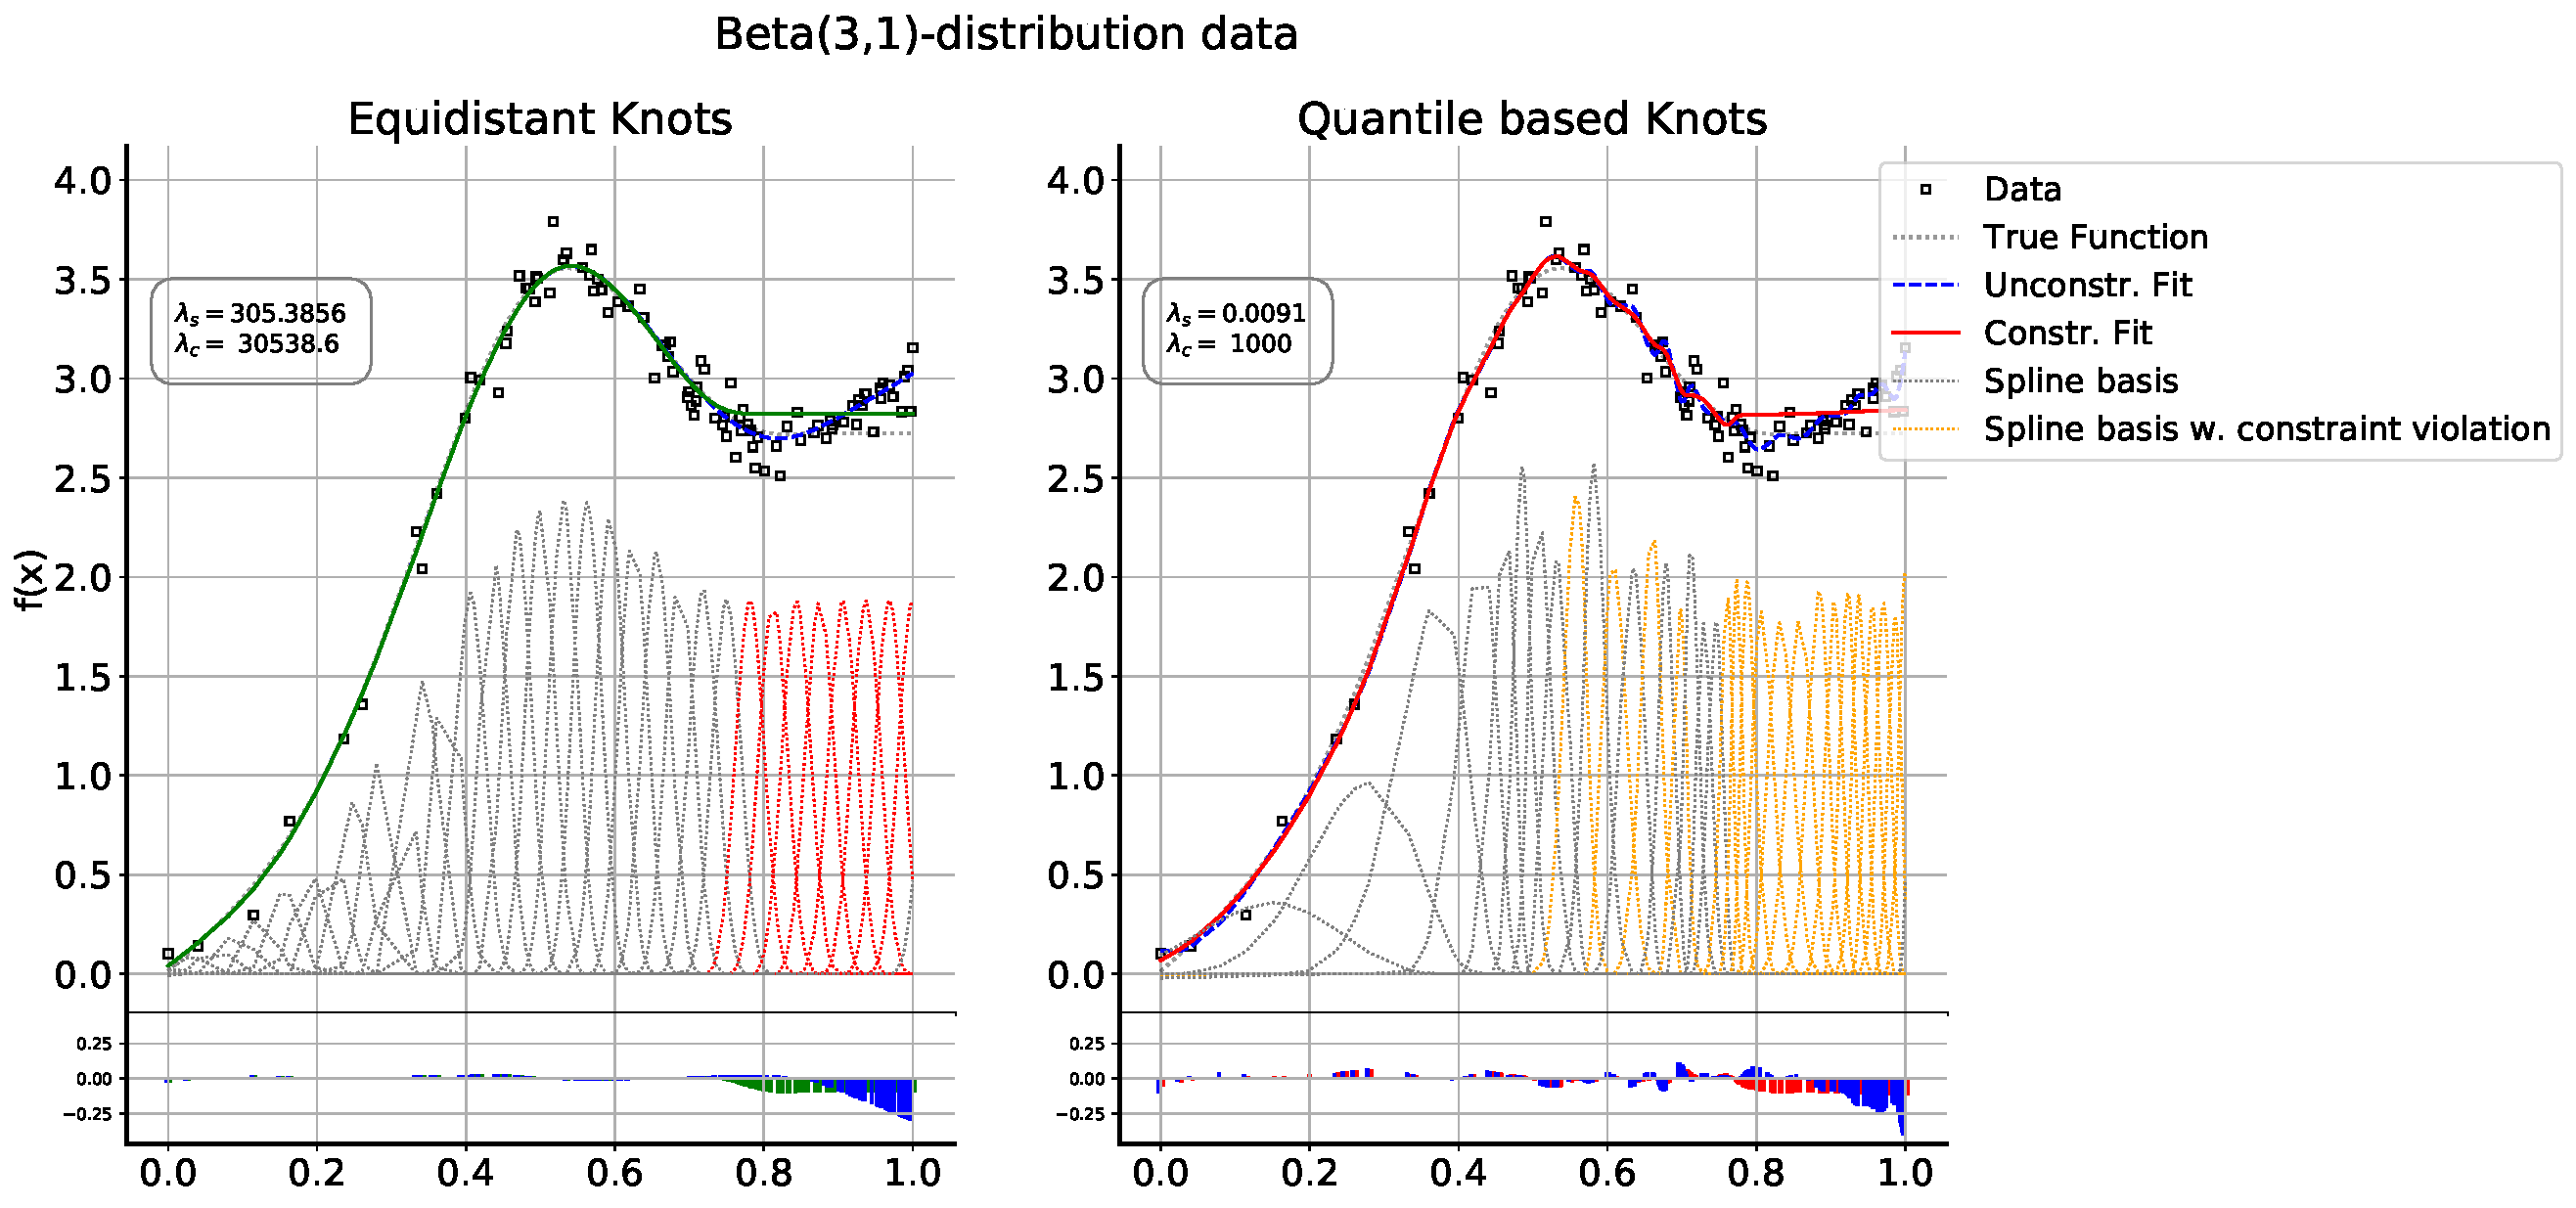
\includegraphics[width=\columnwidth]{../thesisplots/exp_beta/exp_right_skewed_data_ndata_250_rseed_1.pdf}
	\caption{Constr. and unconstr. fit and residuals for right skewed data}
	\label{fig:fit_right_skew_250}
\end{figure}

The smoothing parameters were set to $\lambda_{s, equidistant} = 303.39$ for equidistant knot placement and $\lambda_{s, quantile} = 0.0091$ for quantile based knot placement. The low optimal smoothing parameter again leads to a wiggly estimate  especially for the decreasing part of the quantile based knot placement fit compared the the smooth estimate for equidistant knot placement. This can also be seen in the residual part of Figure \ref{fig:fit_right_skew_250}. The constraint parameters were set to $\lambda_{c, equidistant} = 3053.9$ and $\lambda_{c, quantile} = 9111.6$. The constraint is hold for both knot types, except for $x \approx 0.73$ for quantile based knot placement. Both fits overestimate the level of the constant function part.

The mean squared errors on training and test set as well as the AIC values are given in Table \ref{tab:metrics_53}. The situation is quite similar to the left skewed data experiment and middle skewed data experiment given in the previous chapters. The constraint equidistant model is the overall best model producing the lowest $\text{MSE}_{train}$ and $\text{MSE}_{test}$ as well as AIC value.

\begin{table}[H]
	\centering
	\begin{tabular}{|l|l|l|l|}
		\hline
		\textbf{Model} & \textbf{$\text{MSE}_{train}$} & \textbf{$\text{MSE}_{test}$}  & \textbf{AIC} \\ \hline \toprule
		Unconstraint + E  & $0.89 * 10^{-2}$  & $1.06 * 10^{-2}$ & -253.2       \\ \hline
		Unconstraint + Q  & $1.05 * 10^{-2}$  & $0.99 * 10^{-2}$ & -167.8       \\ \hline
		Constraint + E    & $0.36 * 10^{-2}$  & $0.50 * 10^{-2}$ & -308.3       \\ \hline
		Constraint + Q    & $0.45 * 10^{-2}$  & $0.61 * 10^{-2}$ & -268.2      \\ \hline \bottomrule
	\end{tabular}
	\caption{MSEs and AIC for Exp. 5.3}
	\label{tab:metrics_53}
\end{table}


\subsubsection{Exp. 5.4: Equidistant vs. Quantile Based Knot Placement for Left Skewed Data and Many Data Points}

We will now investigate the effect of non-regular data distributions for Function \ref{eq:test_func_2} in (\ref{eq:test_func_2}) given by a beta distribution with $a = 1$ and $b = 3$, this time using $n=2500$ data points. The fits for equidistant and quantile based knot placement can be seen in Figure \ref{fig:fit_left_skew_2500}. 

\begin{figure}[H]
	\centering
	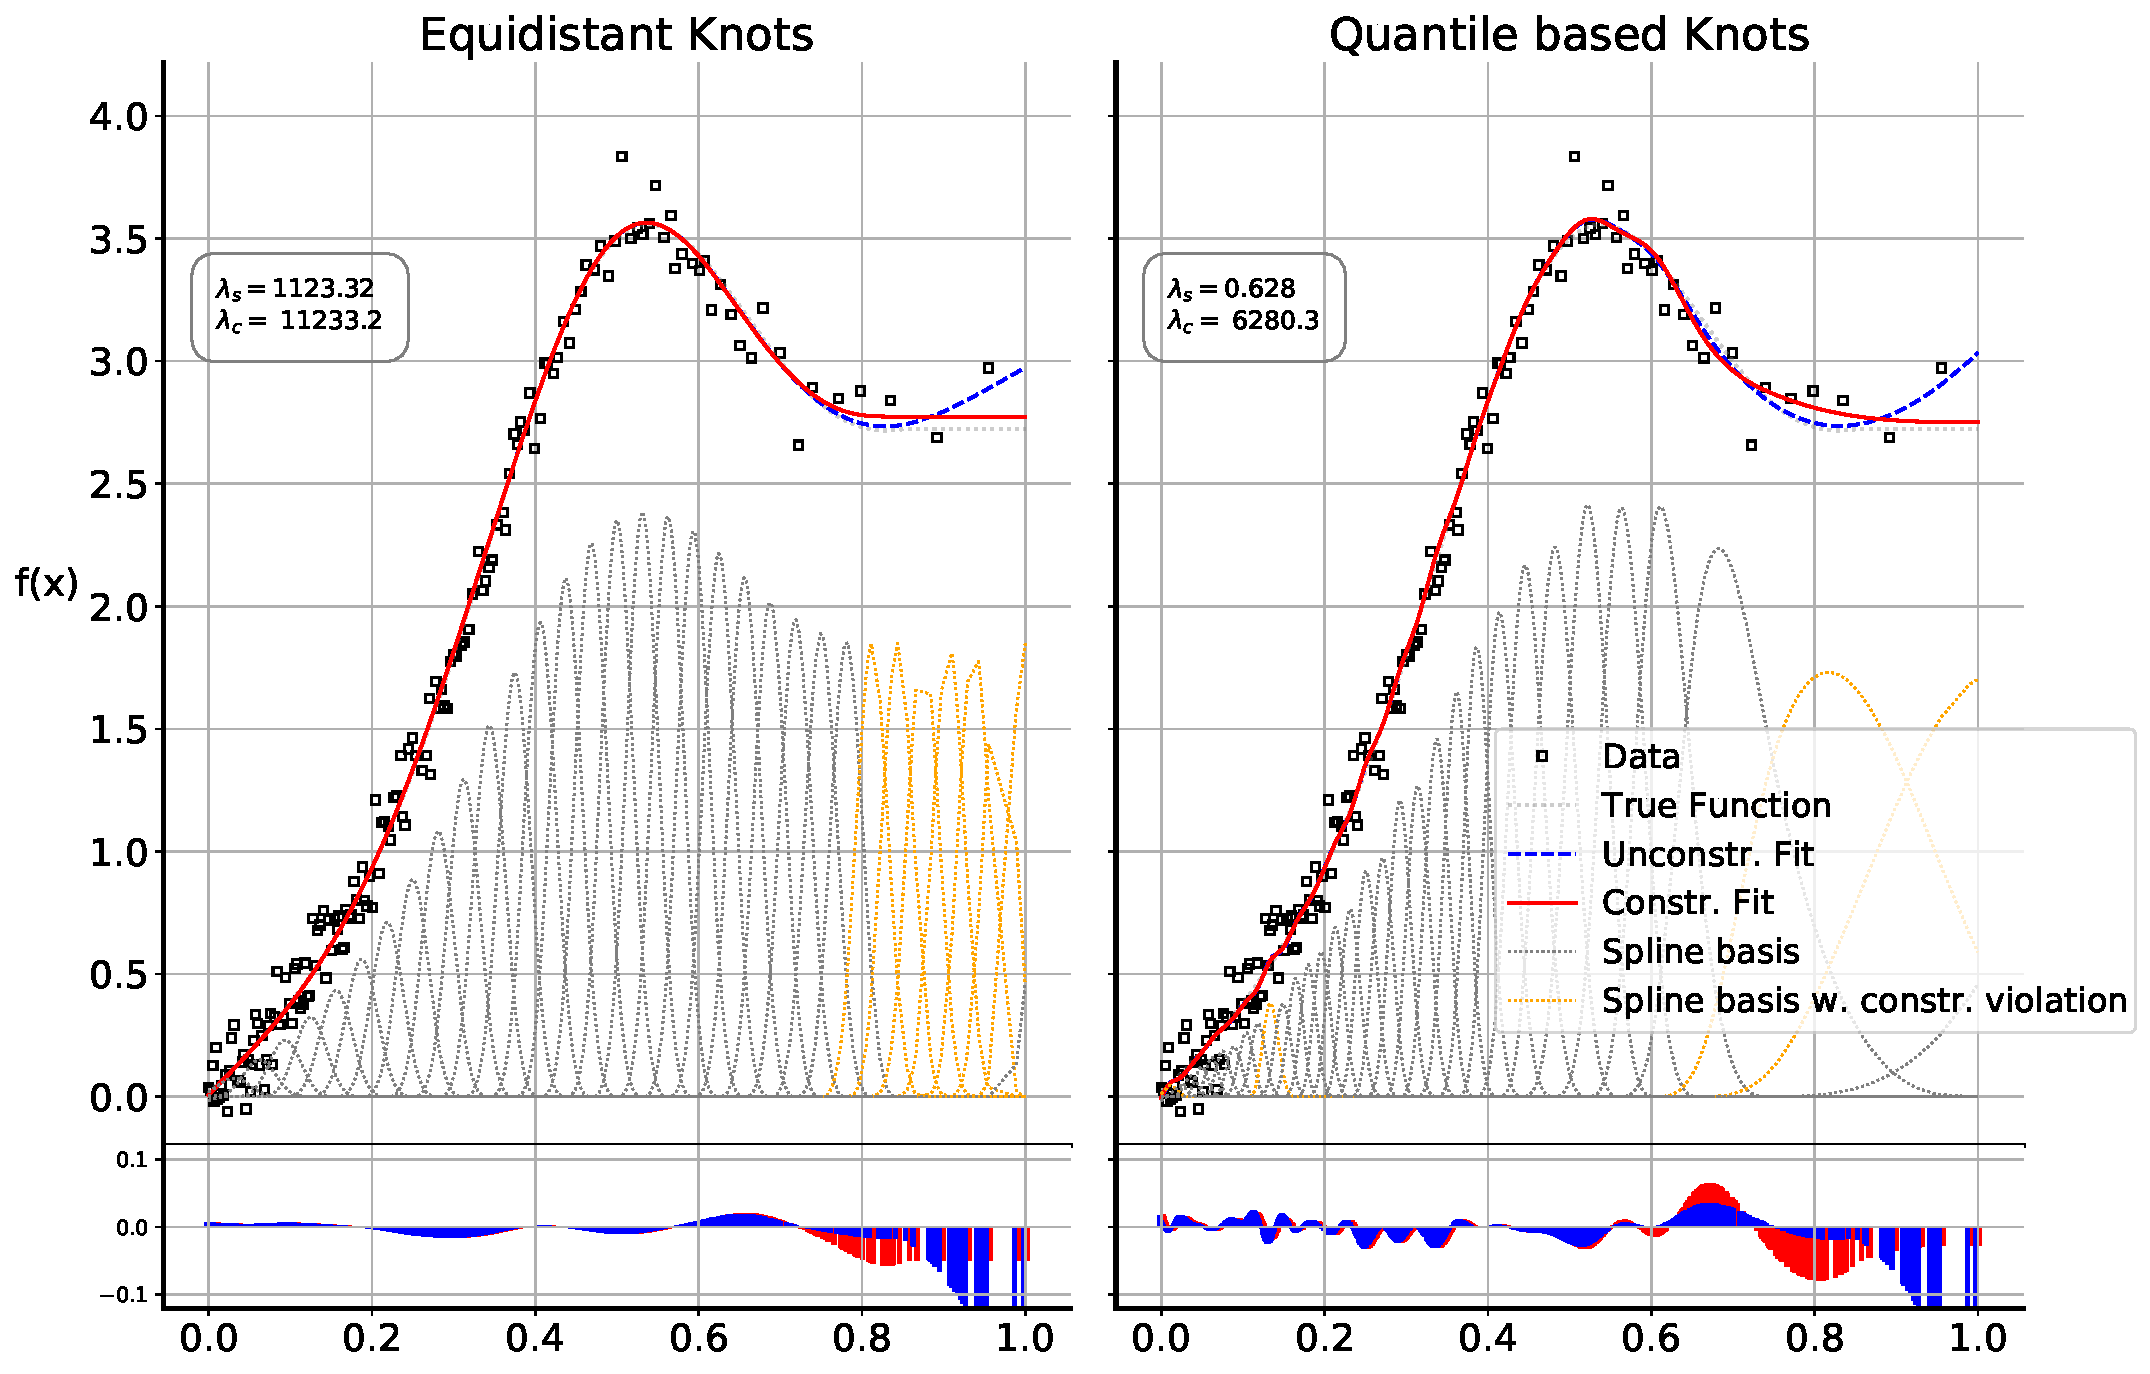
\includegraphics[width=\columnwidth]{../thesisplots/exp_beta/exp_left_skewed_data_ndata_2500_rseed_1.pdf}
	\caption{Constr. and unconstr. fit and residuals for left skewed data}
	\label{fig:fit_left_skew_2500}
\end{figure}

The smoothing parameters were set to $\lambda_{s, equidistant} = 1123.32$ for equidistant knot placement and $\lambda_{s, quantile} = 0.628$ for quantile based knot placement. The constraint parameters were set to $\lambda_{c, equidistant} = 11233.2$ and $\lambda_{c, quantile} = 6280.3$. The constraint is hold for both knot types. Both fits produces a nearly optimal fit especially for the peak region. Using a higher number of data points relaxes the problem of a wiggly estimate for the quantile based knot placement fit. Nevertheless, its residual is higher than for equidistant knot placement.

The mean squared errors on training and test set as well as the AIC values are given in Table \ref{tab:metrics_54}. The situation is similar to the experiment given in the previous chapters. The constraint equidistant model is the overall best model producing the lowest $\text{MSE}_{train}$ and second lowest $\text{MSE}_{test}$ as well as AIC value, while holding the constraint. Using a larger number of data points, the differences between equidistant and quantile based knot placement in terms of accuracy and constraint fidelity nearly vanish. 

\begin{table}[H]
	\centering
	\begin{tabular}{|l|l|l|l|}
		\hline
		\textbf{Model} & \textbf{$\text{MSE}_{train}$} & \textbf{$\text{MSE}_{test}$}  & \textbf{AIC} \\ \hline \toprule
		Unconstraint + E  & $2.25 * 10^{-4}$  & $1.20 * 10^{-4}$ & -5605.4       \\ \hline
		Unconstraint + Q  & $3.76 * 10^{-4}$  & $2.27 * 10^{-4}$ & -5135.1      \\ \hline
		Constraint + E    & $1.29 * 10^{-4}$  & $1.31 * 10^{-4}$ & -5553.9      \\ \hline
		Constraint + Q    & $3.30 * 10^{-4}$  & $3.33 * 10^{-4}$ & -4908.5     \\ \hline \bottomrule
	\end{tabular}
	\caption{MSEs and AIC for Exp. 5.4}
	\label{tab:metrics_54}
\end{table}


In summary, equidistant knot placement produces better fits in terms of smoothness and accuracy for a low number of data points. Its residuals are overall lower than the ones from quantile based knot placement. This comes mostly from the fact that the optimal smoothing parameter for quantile based knot placement is quite low for all experiments compared to the equidistant equivalent. We can therefore conclude that quantile based knot placement for a lower number of data points is not beneficial in terms of fit quality compared to equidistant knot placement. Further, we can conclude that the incorporation of a priori domain knowledge improves the qualitative and quantitative behavior of the fit even in situations where the data is not well distributed.  


\subsection{Exp. 6: Real life data} \label{subsec:real-life-data}

We will now try to incorporate a priori domain knowledge in the fitting process using real-life data. The data is generated from a heat treatment process of aluminum. The aluminum is heated to a specific temperature and then cooled using water jets.

We try to estimate the heat transfer coefficient $\alpha := \alpha(T, \dot m)$ as a function of the temperature $T$ and the mass flow $\dot m$. We know beforehand, that the heat transfer coefficient $\alpha$ may only increase when increasing the mass flow $\dot m$ and that it shows a peak behavior for increasing temperature $T$. 

A further problem is the data situation given in Figure \ref{fig:ebner_data_situation}. Here we show how many data points are given in a area of approximately $50 K$ and $0.9 [kg/s]$. We have some regions, where no data is available, while the majority of data points is located in small areas.


\begin{figure}[H]
	\centering
	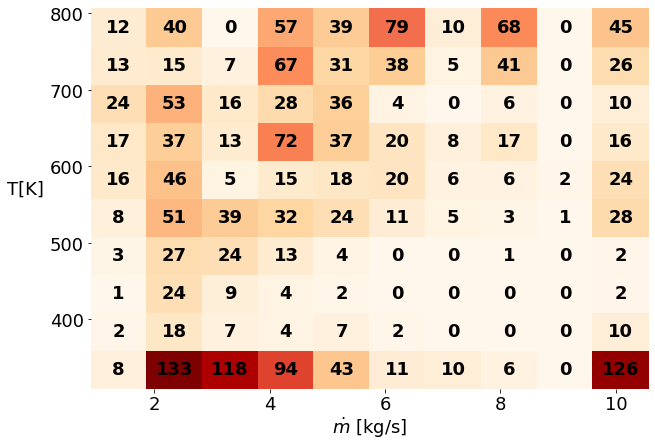
\includegraphics[width=\columnwidth]{../thesisplots/ebner/data_distribution.png}
	\caption{Data Situation}
	\label{fig:ebner_data_situation}
\end{figure}

We use the additive model ansatz using two spline models, $s_1(T)$ and $s_2(\dot m)$, and constrain $s_1(T)$ by the unimodality constraint and $s_2(\dot m)$ by the increasing constraint. We use $k=50$ splines for both. The smoothing parameters were set to $\lambda_{s, s_1} = 908.52$ and $\lambda_{s, s_2} = 383.12$. The constraint parameters were set to $\lambda_{c, s_1} = 9085.2$ and $\lambda_{c, s_2} = 3831.2$. The fit using the a priori domain knowledge is given in Figure \ref{fig:ebner_fit_s250}. The unconstrained fit is given in Figure \ref{fig:ebner_fit_unc_s250}. 

\begin{figure}[H]
	\centering
	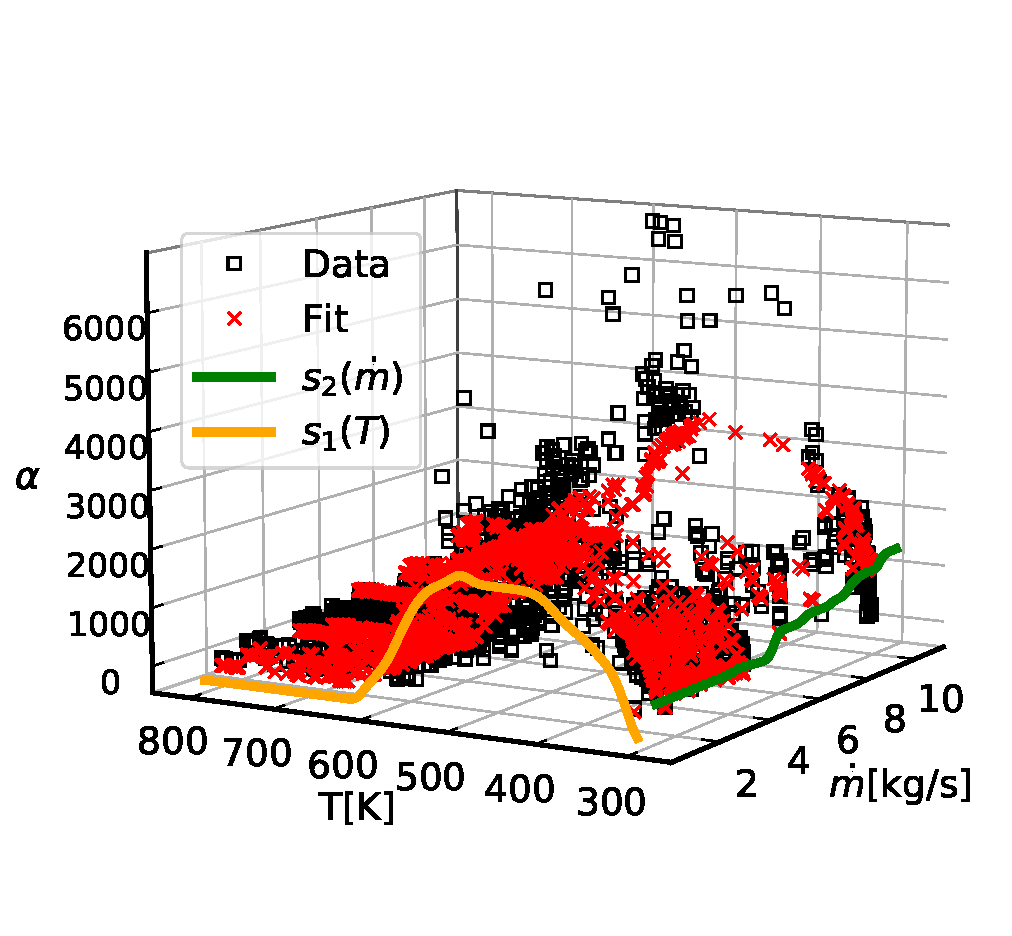
\includegraphics[width=\columnwidth]{../thesisplots/ebner/Model_constraint_lam_s1_383_lam_s2_908.pdf}
	\caption{Constr. fit for real-life data}
	\label{fig:ebner_fit_s250}
\end{figure}

\begin{figure}[H]
	\centering
	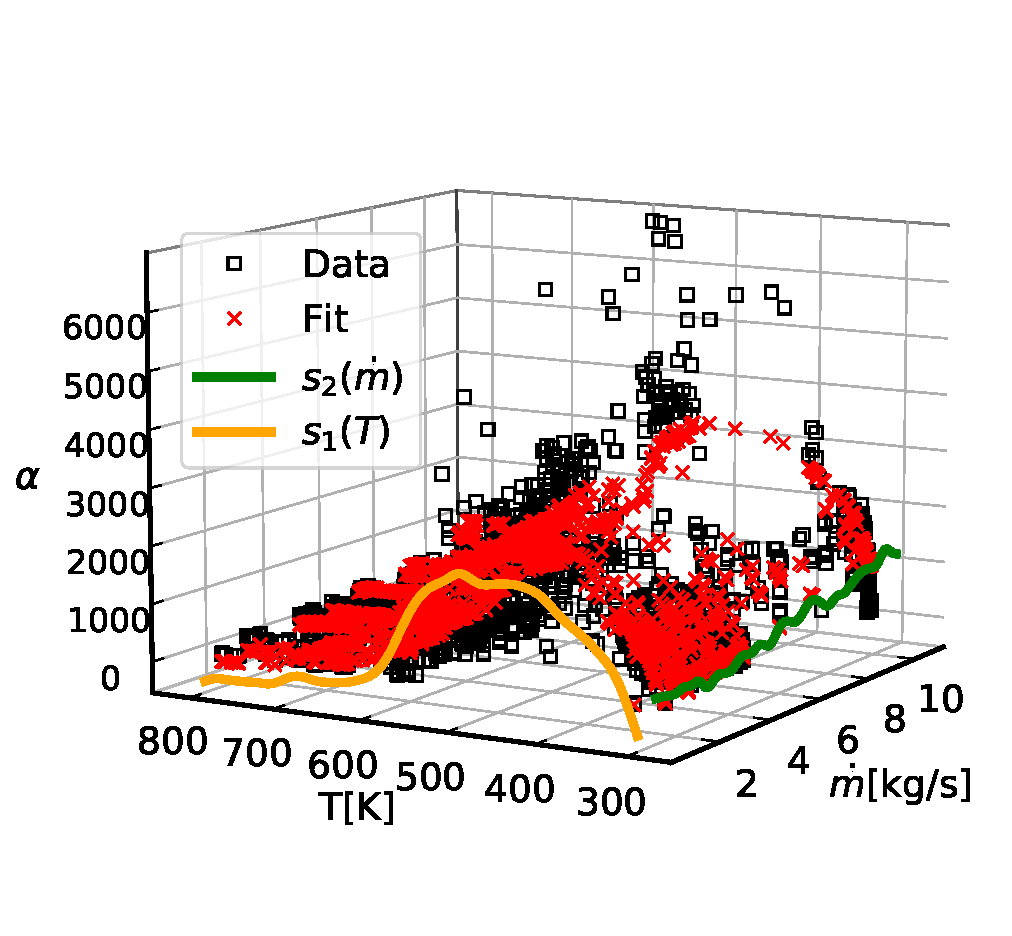
\includegraphics[width=\columnwidth]{../thesisplots/ebner/Model_unc_lam_s1_383_lam_s2_908.pdf}
	\caption{Unconstr. fit for real-life data}
	\label{fig:ebner_fit_unc_s250}
\end{figure}


The a priori domain knowledge is hold quite well for the constraint fit given in Figure \ref{fig:ebner_fit_s250}. In comparison, the unconstraint fit using the same smoothing parameters is given in Figure \ref{fig:ebner_fit_unc_s250}. Here, especially the mass flow dependent function $s_2(\dot m)$ does not hold the constraint of being increasing. The temperature dependent function $s_1(T)$ is quite smooth, but also violates the unimodality constraint for $T \approx 700 \text{K}$ and $T \approx 450 \text{K}$. 

The mean squared errors and AIC values for both fits are shown in Table \ref{tab:metrics_6}. The constraint fit has lower $\text{MSE}_{train}$ and $\text{MSE}_{test}$ as well as AIC value. 


\begin{table}[H]
	\centering
	\begin{tabular}{|l|l|l|l|}
		\hline
		\textbf{Model} & \textbf{$\text{MSE}_{train}$} & \textbf{$\text{MSE}_{test}$}  & \textbf{AIC} \\ \hline \toprule
		Unconstraint  & $1.5178 * 10^{6}$  & $1.3843 * 10^{6}$ & 2748.5      \\ \hline
		Constraint    & $1.5161 * 10^{6}$  & $1.3808 * 10^{6}$ & 2723.9      \\ \hline
	\end{tabular}
	\caption{MSEs and AIC for Exp. 6}
	\label{tab:metrics_6}
\end{table}


\section{Summary}

The incorporation of a priori domain knowledge in the fitting process using structured additive regression, B-splines, a smoothness penalty and a user-defined constraint penalty is possible for simulated and real-life data. The use of a priori domain knowledge improves the quality of the fit and makes the estimation process more robust against noise, data outliers and measurements errors. 


\end{document}